\documentclass[11pt]{book}

% praeambel.tex — Hamilton-Jacobi-kompendiet
% Den sædvanlige opsætning (jf. lineær algebra- og kvantemekanik-kompendierne)

\usepackage[a4paper,twoside,margin=2.5cm]{geometry}
\usepackage[danish]{babel}
\usepackage[utf8]{inputenc}
\usepackage[T1]{fontenc}
\usepackage{mathpazo}
\usepackage{amsmath,amssymb,amsthm}
\usepackage{physics}
\usepackage{graphicx}
\usepackage{tikz}
\usetikzlibrary{arrows.meta,calc,positioning,decorations.pathmorphing}
\usepackage{mdframed}
\usepackage{fancyhdr}
\usepackage{hyperref}
\usepackage{caption}
\captionsetup{font=small,margin=1.2cm}

% --- Sidehoved/-fod (even/odd) ---
\pagestyle{fancy}
\fancyhf{}
\fancyhead[LE,RO]{\thepage}
\fancyhead[RE]{\leftmark}
\fancyhead[LO]{\rightmark}
\renewcommand{\headrulewidth}{0.4pt}

% --- Farvede miljøer ---
\newmdenv[linecolor=blue!60!black,backgroundcolor=blue!5,linewidth=1pt,roundcorner=3pt]{eksempel}
\newmdenv[linecolor=orange!70!black,backgroundcolor=orange!5,linewidth=1pt,roundcorner=3pt]{bemaerkning}
\newmdenv[linecolor=orange!70!black,backgroundcolor=orange!5,linewidth=1pt,roundcorner=3pt]{opgave}

% --- Faste makroer (videreføres fra tidligere kompendier, udvides efter behov) ---
% \newcommand{\pd}[2]{\frac{\partial #1}{\partial #2}}
% Hamilton-Jacobi-specifikke makroer tilføjes her efterhånden som de opstår,
% f.eks. \newcommand{\Ham}{\mathcal{H}} for Hamilton-funktionen,
% \newcommand{\Lag}{\mathcal{L}} for Lagrange-funktionen,
% \newcommand{\Hact}{S} for virkningsfunktionen (Hamiltons principfunktion).


\title{Hamilton-Jacobi-kompendiet}
\author{Jørn Skoven Pedersen}
\date{}

\begin{document}

\frontmatter
\maketitle
\tableofcontents

\mainmatter

% --- Del I: Lagrange- og Hamilton-mekanik ---
\part{Lagrange- og Hamilton-mekanik}
% kap01.tex — Newtonsk mekanik og variationsprincipper
% Hamilton-Jacobi-kompendiet

\chapter{Newtonsk mekanik og variationsprincipper}
\label{kap:newton-variation}

\section{Hvorfor forlade Newton?}

Newtons anden lov,
\begin{equation}
  \vb{F} = m\vb{a},
\end{equation}
er det mest direkte udtryk for mekanikkens grundlov, vi har. Den er lokal
i tid, den er intuitiv, og den virker for et enkelt punkt uden
tvangsbetingelser. Men så snart vi vender os mod systemer, hvor
bevægelsen er begrænset af tvang — en kugle der ruller på en skinne, en
pendul der hænger i en stiv stang, en gasmolekyle der er låst inde i en
beholder — bliver Newtons formulering upraktisk. Problemet er ikke, at
loven svigter; problemet er, at den kræver, at vi kender \emph{alle}
kræfter, herunder de tvangskræfter (normalkræfter, snortræk, reaktioner
fra skinner), der holder systemet på dets tilladte bane. Disse
tvangskræfter udfører intet arbejde i den retning, bevægelsen faktisk
sker i, og de er i praksis ofte netop det, vi \emph{ikke} kender og
\emph{ikke} er interesserede i.

Kapitlets mål er at motivere og udlede et alternativt udgangspunkt —
D'Alemberts princip — der elegant elimininerer tvangskræfterne fra
beskrivelsen, uden at vi behøver kende deres størrelse. Dette er første
skridt på vejen til Lagrange- og senere Hamilton-formalismen
(kapitel~\ref{kap:lagrange} og \ref{kap:hamilton}), som igen er
forudsætningen for Hamilton-Jacobi-teorien, der er kompendiets egentlige
mål.

Den fysiske pointe, vi skal holde fast i hele vejen igennem, er denne:
\emph{et system med tvangsbetingelser har færre uafhængige
frihedsgrader end antallet af koordinater, vi nemmest kan nedskrive
det i}. Kunsten er at finde en beskrivelse, der kun bruger de
uafhængige frihedsgrader — og det er præcis, hvad generaliserede
koordinater giver os.

\section{Frihedsgrader og generaliserede koordinater}

Betragt et system af $N$ punktpartikler. Uden tvangsbetingelser har
systemet $3N$ frihedsgrader — de kartesiske koordinater
$\vb{r}_1,\dots,\vb{r}_N$. Er systemet underlagt $k$ uafhængige
tvangsbetingelser, reduceres antallet af uafhængige frihedsgrader til
\begin{equation}
  n = 3N - k.
\end{equation}

I stedet for at arbejde med de $3N$ kartesiske koordinater og $k$
tvangsligninger, indfører vi $n$ \emph{generaliserede
koordinater}\index{generaliserede koordinater}
$q_1,\dots,q_n$, valgt så tvangsbetingelserne er automatisk opfyldt for
alle værdier af $q_i$. De kartesiske koordinater kan da skrives som
funktioner af de generaliserede koordinater (og eventuelt tiden, hvis
tvangsbetingelserne selv er tidsafhængige):
\begin{equation}
  \vb{r}_\alpha = \vb{r}_\alpha(q_1,\dots,q_n,t), \qquad \alpha = 1,\dots,N.
  \label{eq:transformationsligning}
\end{equation}

\begin{eksempel}
For et simpelt plant pendul af længde $\ell$, der svinger i en fast
lodret plan, er den naturlige kartesiske beskrivelse $(x,y)$ med
tvangsbetingelsen $x^2+y^2=\ell^2$: to koordinater, én
tvangsbetingelse, altså $n = 2-1=1$ frihedsgrad. Vi vælger den
generaliserede koordinat $q_1=\theta$, udslagsvinklen fra lodret, og
skriver
\begin{equation}
  x = \ell\sin\theta, \qquad y = -\ell\cos\theta.
\end{equation}
Tvangsbetingelsen $x^2+y^2=\ell^2$ er nu automatisk opfyldt for
\emph{alle} værdier af $\theta$ — vi behøver aldrig nedskrive den igen.
\end{eksempel}

Denne idé — at vælge koordinater, hvori tvangsbetingelserne er ``bygget
ind'' — er selve nøglen til alt, hvad der følger i dette kompendium.

\subsection{Holonome og ikke-holonome tvangsbetingelser}

En tvangsbetingelse, der kan skrives som en ligning i koordinaterne (og
eventuelt tiden),
\begin{equation}
  f(\vb{r}_1,\dots,\vb{r}_N,t) = 0,
\end{equation}
kaldes \emph{holonom}\index{tvangsbetingelse!holonom}\index{holonom tvangsbetingelse|see{tvangsbetingelse, holonom}}. Pendulets $x^2+y^2-\ell^2=0$ er et eksempel.
Holonome tvangsbetingelser er netop dem, der kan elimineres ved et
koordinatvalg som i \eqref{eq:transformationsligning}: de reducerer
antallet af \emph{koordinater}, vi behøver.

En tvangsbetingelse, der ikke kan skrives på denne form — typisk fordi
den kun begrænser hastigheder uden at være en totale-differential af
en funktion af koordinaterne — kaldes \emph{ikke-holonom}\index{tvangsbetingelse!ikke-holonom}. Det klassiske
eksempel er en mønt, der ruller uden at glide på et plan: mønten kan nå
et hvilket som helst punkt på planet med en hvilken som helst
orientering, men rullebetingelsen (ingen glidning) lægger et
øjeblikkeligt bånd på hastighedsvektoren, som ikke integrerer til et
enkelt bånd på positionen.

I dette kompendium beskæftiger vi os \emph{udelukkende} med holonome
tvangsbetingelser. Det er ikke en indskrænkning, der koster os noget
væsentligt: næsten alle systemer, der er relevante for vejen mod
Hamilton-Jacobi-teori og kvantisering, er holonome, og den formelle
maskine (Lagrange- og Hamilton-formalismen), vi bygger op, forudsætter
det.

\section{Virtuel forskydning og virtuelt arbejde}

For at komme fra Newtons love til et princip, der ikke kræver kendskab
til tvangskræfterne, indfører vi begrebet \emph{virtuel
forskydning}\index{virtuel forskydning}.

En virtuel forskydning $\delta\vb{r}_\alpha$ er en tænkt,
infinitesimal ændring af partikel $\alpha$'s position, som

\begin{itemize}
  \item er i overensstemmelse med tvangsbetingelserne på det givne
        tidspunkt $t$ (systemet ``flyttes'' til en anden tilladt
        konfiguration),
  \item sker \emph{momentant} — tiden holdes fast, $\delta t = 0$ — i
        modsætning til en virkelig forskydning $d\vb{r}_\alpha$, som
        sker i løbet af et tidsinterval $dt$, og som derfor kan
        involvere tidsafhængigheden i tvangsbetingelserne selv.
\end{itemize}

Ordet ``virtuel'' markerer netop denne forskel: $\delta\vb{r}_\alpha$ er
ikke en bevægelse, systemet rent faktisk udfører, men en tilladt
\emph{sammenligningskonfiguration}, vi bruger som redskab.

\emph{Virtuelt arbejde}\index{virtuelt arbejde} er det arbejde, en kraft $\vb{F}_\alpha$ ville
udføre under en sådan virtuel forskydning:
\begin{equation}
  \delta W = \sum_{\alpha} \vb{F}_\alpha \cdot \delta\vb{r}_\alpha.
\end{equation}

Den centrale egenskab, vi skal udnytte, er denne: for et system med
\emph{ideale} tvangsbetingelser — dvs.\ tvangsbetingelser, hvis
tvangskræfter $\vb{R}_\alpha$ står vinkelret på enhver tilladt virtuel
forskydning — gælder
\begin{equation}
  \sum_\alpha \vb{R}_\alpha \cdot \delta\vb{r}_\alpha = 0.
  \label{eq:ideal-tvang}
\end{equation}
Dette er ikke en tilfældig antagelse; det er selve definitionen af, at
en tvangsbetingelse er ``glat'' i den forstand, vi har brug for: en
normalkraft fra en glat skinne, spændingen i en stiv, uelastisk snor,
eller reaktionen fra en glat flade opfylder alle \eqref{eq:ideal-tvang},
fordi de netop er rettet vinkelret på de bevægelser, tvangen tillader.
Friktion opfylder den derimod \emph{ikke} i almindelighed — det er
grunden til, at friktion kræver særlig behandling i denne formalisme
(se bemærkningen nedenfor).

\begin{bemaerkning}
Idealiteten \eqref{eq:ideal-tvang} er den fysiske forudsætning, hele
det følgende bygger på. Den er ikke en matematisk trivialitet, men et
udsagn om, hvilke kræfter naturen rent faktisk lader tvangsbetingelser
udøve. At normalkræfter og snortræk opfylder den, skyldes, at de er
\emph{reaktionskræfter}: de justerer sig præcis til den størrelse, der
er nødvendig for at holde tvangen, og ingen mere — de har intet ``eget''
bidrag til bevægelsesenergien langs de tilladte retninger. Friktion er
anderledes, fordi dens størrelse ikke blot bestemmes af tvangen selv,
men af den relative bevægelse; den formalisme, vi bygger her, dækker
derfor konservative systemer og systemer med ideale tvangsbetingelser,
men skal udvides (typisk med Rayleighs dissipationsfunktion) for at
håndtere friktion. Vi kommer ikke til at have brug for dette i resten
af kompendiet.
\end{bemaerkning}

\section{D'Alemberts princip}

Newtons anden lov for partikel $\alpha$ lyder
\begin{equation}
  \vb{F}_\alpha^{(a)} + \vb{R}_\alpha = m_\alpha\ddot{\vb{r}}_\alpha,
\end{equation}
hvor vi har opdelt den samlede kraft i en \emph{anvendt} (påtrykt) kraft
$\vb{F}_\alpha^{(a)}$ — tyngdekraft, fjederkraft, elektrisk kraft, osv.
— og tvangskraften $\vb{R}_\alpha$. Omskrevet:
\begin{equation}
  \vb{F}_\alpha^{(a)} - m_\alpha\ddot{\vb{r}}_\alpha = -\vb{R}_\alpha.
\end{equation}
Vi ganger begge sider skalært med en virtuel forskydning
$\delta\vb{r}_\alpha$ og summerer over alle partikler:
\begin{equation}
  \sum_\alpha \left(\vb{F}_\alpha^{(a)} - m_\alpha\ddot{\vb{r}}_\alpha\right)\cdot\delta\vb{r}_\alpha
  = -\sum_\alpha \vb{R}_\alpha\cdot\delta\vb{r}_\alpha.
\end{equation}
Ifølge \eqref{eq:ideal-tvang} er højresiden nul for ideale
tvangsbetingelser. Vi står tilbage med \emph{D'Alemberts
princip}\index{D'Alemberts princip}:
\begin{equation}
  \boxed{\sum_\alpha \left(\vb{F}_\alpha^{(a)} - m_\alpha\ddot{\vb{r}}_\alpha\right)\cdot\delta\vb{r}_\alpha = 0.}
  \label{eq:dalembert}
\end{equation}

Dette er den afgørende pointe i kapitlet: tvangskræfterne
$\vb{R}_\alpha$ er \emph{helt forsvundet} fra formuleringen. Vi behøver
ikke kende dem for at bruge \eqref{eq:dalembert} — kun de anvendte
kræfter og de tilladte virtuelle forskydninger, som selv er bestemt af
tvangsbetingelsernes geometri.

\begin{bemaerkning}
D'Alemberts princip kaldes ofte ``det generaliserede princip om virtuelt
arbejde'', fordi det udvider den statiske ligevægtsbetingelse
$\sum_\alpha \vb{F}_\alpha^{(a)}\cdot\delta\vb{r}_\alpha = 0$ (velkendt
fra statik: et system er i ligevægt, hvis det virtuelle arbejde af de
anvendte kræfter er nul for alle tilladte virtuelle forskydninger) til
dynamiske systemer, ved at behandle $-m_\alpha\ddot{\vb{r}}_\alpha$ som
en ekstra ``inertikraft''. Denne omtolkning — at accelerationen kan
regnes med som en kraft, der modvirker bevægelsen — er den samme idé,
man møder som ``d'Alembert-kraft'' eller (i mere kavaleret sprogbrug)
``centrifugalkraft'' i roterende referencesystemer.
\end{bemaerkning}

\section{Eksempel: kloden på et glat skråplan}

Lad os se D'Alemberts princip i arbejde på et konkret eksempel, før vi
går videre til den generelle omskrivning i generaliserede koordinater
(kapitel~\ref{kap:lagrange}).

\begin{eksempel}
En kugle med masse $m$ glider uden friktion ned langs et fast skråplan
med hældningsvinkel $\alpha$ (se figur~\ref{fig:skraaplan}). Lad $s$
være afstanden målt langs planet fra toppen. Tvangsbetingelsen er, at
kuglen forbliver på planets overflade; den eneste frihedsgrad er $s$.

Den anvendte kraft er tyngden, $\vb{F}^{(a)} = -mg\,\hat{\vb{y}}$. En
virtuel forskydning langs planet er $\delta\vb{r} = \delta s\,\hat{\vb{s}}$,
hvor $\hat{\vb{s}}$ er enhedsvektoren langs planet, med komponenter
$(\cos\alpha, -\sin\alpha)$ i det viste koordinatsystem.

Kuglens acceleration er $\ddot{\vb{r}} = \ddot{s}\,\hat{\vb{s}}$ (planet
er fast, så bevægelsen er ren translation langs $\hat{\vb{s}}$).
D'Alemberts princip \eqref{eq:dalembert} giver
\begin{equation}
  \left(\vb{F}^{(a)} - m\ddot{\vb{r}}\right)\cdot\delta\vb{r} = 0
  \quad\Longrightarrow\quad
  \left(-mg\,\hat{\vb{y}} - m\ddot{s}\,\hat{\vb{s}}\right)\cdot\hat{\vb{s}}\,\delta s = 0.
\end{equation}
Da $\delta s$ er arbitrær (og ikke-nul), må parentesen selv være nul:
\begin{equation}
  -mg\,\hat{\vb{y}}\cdot\hat{\vb{s}} - m\ddot{s} = 0
  \quad\Longrightarrow\quad
  \ddot{s} = -g\,\hat{\vb{y}}\cdot\hat{\vb{s}} = g\sin\alpha,
\end{equation}
hvor vi har brugt $\hat{\vb{y}}\cdot\hat{\vb{s}} = -\sin\alpha$ ud fra
komponenterne ovenfor. Vi genfinder det velkendte resultat
$\ddot{s}=g\sin\alpha$ — men bemærk, at vi \emph{aldrig} har skullet
opskrive normalkraften $N$ fra planet på kuglen. Den er elimineret
fuldstændigt, fordi den (ideelt) ikke udfører virtuelt arbejde langs
den tilladte bevægelse.
\end{eksempel}

\begin{figure}[htbp]
  \centering
  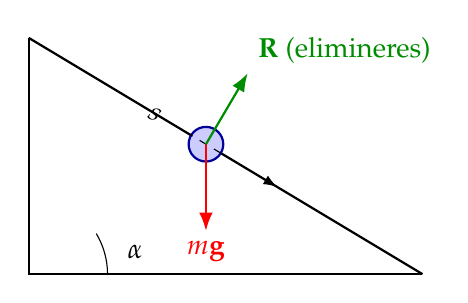
\begin{tikzpicture}[scale=1.0]
    % Skråplan
    \draw[thick] (0,3) -- (0,0) -- (5,0);
    \draw[thick] (0,3) -- (5,0);
    % Vinkelmarkering
    \draw (1.0,0) arc (0:31:1.0);
    \node at (1.35,0.28) {$\alpha$};
    % Kugle på planet
    \pgfmathsetmacro{\sfrac}{0.45}
    \coordinate (P) at ({5*\sfrac},{3*(1-\sfrac)});
    \filldraw[fill=blue!20,draw=blue!60!black,thick] (P) circle (0.22);
    % s-akse langs planet
    \draw[-{Latex},dashed] (0,3) -- ($(P)+(0.9,-0.54)$);
    \node[rotate=-31] at ($(0,3)+(1.6,-0.97)$) {$s$};
    % Tyngdekraft
    \draw[-{Latex},thick,red] (P) -- ++(0,-1.1) node[below] {$m\vb{g}$};
    % Normalkraft (elimineres i D'Alembert, men vist for reference)
    \draw[-{Latex},thick,green!55!black] (P) -- ++(0.53,0.90) node[above right] {$\vb{R}$ (elimineres)};
  \end{tikzpicture}
  \caption{Kugle på et glat skråplan. Tyngden $m\vb{g}$ er den anvendte
  kraft; tvangskraften (normalkraften) $\vb{R}$ udfører intet virtuelt
  arbejde langs den tilladte bevægelse $\delta s$ og forsvinder derfor
  fra D'Alemberts princip.}
  \label{fig:skraaplan}
\end{figure}

\section{Fra D'Alembert til et variationsprincip}

D'Alemberts princip \eqref{eq:dalembert} er stadig formuleret i
kartesiske koordinater og vektorielt sprog. Det er et vigtigt
mellemtrin, men ikke slutdestinationen. To ting gør det utilfredsstillende
som slutformulering:

\begin{enumerate}
  \item Det er stadig udtrykt via de $3N$ kartesiske koordinater
        $\vb{r}_\alpha$, ikke via de $n$ uafhængige generaliserede
        koordinater $q_i$, som faktisk beskriver systemets frihedsgrader.
  \item Det er et \emph{differentielt} princip: det udtaler sig om
        systemets tilstand ved ét tidspunkt $t$ ad gangen.
\end{enumerate}

Den anden pointe peger frem mod noget dybere. Der findes en anden
klasse af principper i fysikken — \emph{variationsprincipper} — der i
stedet udtaler sig om hele banen $\vb{r}_\alpha(t)$ fra et starttidspunkt
$t_1$ til et sluttidspunkt $t_2$ på én gang, og udpeger den faktiske
bane som den, der gør en bestemt størrelse (et \emph{integral} over
banen) stationær i forhold til alle ``nærliggende'' tænkte baner.

Det klassiske forbillede er Fermats princip i optikken: lysets faktiske
vej mellem to punkter er den, der gør den optiske gangtid stationær
(typisk minimal) i forhold til alle andre tænkte veje. Fermats princip
forudsiger både retlinet forplantning i homogene medier \emph{og}
brydningsloven ved en grænseflade — alt sammen fra ét og samme
udsagn om et integral. Spørgsmålet, vi arbejder os frem mod i
kapitel~\ref{kap:lagrange}, er, om der findes et analogt princip for
mekanisk bevægelse: findes der en størrelse, hvis integral over banen
er stationært netop for den bane, partiklen faktisk følger?

Svaret er ja, og det er netop \emph{Hamiltons
princip}\index{Hamiltons princip}: den faktiske
bane gør \emph{virkningen}\index{virkning (Hamiltons principfunktion)}
\begin{equation}
  S = \int_{t_1}^{t_2} L\,dt
\end{equation}
stationær, hvor $L$ er Lagrange-funktionen\index{Lagrange-funktion}. At D'Alemberts princip —
et differentielt, øjeblik-for-øjeblik-udsagn — faktisk er
\emph{ækvivalent} med et globalt variationsprincip af denne type, er et
af de smukkeste resultater i klassisk mekanik, og det er hovedemnet i
kapitel~\ref{kap:lagrange}, hvor vi udleder Euler-Lagrange-ligningerne
både fra D'Alemberts princip og fra variationsregning direkte.

\begin{bemaerkning}
Det er værd at bemærke allerede her, hvor langt dette fører: netop
fordi Hamiltons princip er formuleret som et udsagn om \emph{hele
banen} snarere end om kræfter ved et enkelt tidspunkt, er det denne
formulering — ikke Newtons love direkte — der generaliserer smukkest
til kvantemekanikken. Feynmans sti-integral-formulering af
kvantemekanikken (som vi vender tilbage til i kapitel~\ref{kap:felter}
og i det senere kompendium om kvantefeltteori) bygger direkte på
virkningsintegralet $S$ og på selve idéen om at summere over
``nærliggende baner''. Variationsprincippet er altså ikke blot en elegant
omskrivning af Newtons mekanik — det er den formulering, der faktisk
overlever overgangen til kvanteteorien.
\end{bemaerkning}

\section{Opsummering}

\begin{itemize}
  \item Newtons love er lokale og kræver kendskab til tvangskræfter,
        som ofte er uinteressante og ukendte.
  \item Holonome tvangsbetingelser kan elimineres ved valg af
        generaliserede koordinater $q_1,\dots,q_n$ ($n$ = systemets
        antal frihedsgrader).
  \item Virtuelle forskydninger $\delta\vb{r}_\alpha$ er momentane,
        tilladte tænkte forskydninger ($\delta t = 0$).
  \item For ideale tvangsbetingelser udfører tvangskræfterne intet
        virtuelt arbejde: $\sum_\alpha \vb{R}_\alpha\cdot\delta\vb{r}_\alpha=0$.
  \item Dette fører til D'Alemberts princip,
        $\sum_\alpha(\vb{F}_\alpha^{(a)}-m_\alpha\ddot{\vb{r}}_\alpha)\cdot\delta\vb{r}_\alpha=0$,
        hvori tvangskræfterne er elimineret.
  \item D'Alemberts princip er stadig kartesisk og differentielt i
        tid. Det næste skridt — kapitel~\ref{kap:lagrange} — er at
        omskrive det i generaliserede koordinater (Lagrange-formalismen)
        og at vise, at det er ækvivalent med et globalt
        variationsprincip (Hamiltons princip), som er den formulering,
        der peger frem mod Hamilton-Jacobi-teori og senere
        kvantisering.
\end{itemize}

\begin{opgave}
Genudled resultatet $\ddot{s}=g\sin\alpha$ fra eksemplet i
afsnit~\ref{eq:dalembert}'s eksempel ved direkte brug af Newtons anden
lov med en eksplicit normalkraft $N$, og overbevis dig om, at $N$ falder
ud af regningen på samme måde, som den gjorde i D'Alembert-formuleringen
— blot ved en ekstra linje udregning i stedet for slet ikke at optræde.
\end{opgave}

\begin{opgave}
Betragt en perle af masse $m$, der er tvunget til at bevæge sig på en
fast, glat, lodret cirkulær ring med radius $R$, under indflydelse af
tyngden. Indfør vinklen $\theta$ målt fra ringens laveste punkt som
generaliseret koordinat, opskriv den tilladte virtuelle forskydning
$\delta\vb{r}$ i retning af $\theta$, og brug D'Alemberts princip til
at udlede bevægelsesligningen for $\theta(t)$.
\end{opgave}

% kap02.tex — Lagrange-formalisme
% Hamilton-Jacobi-kompendiet

\chapter{Lagrange-formalisme}
\label{kap:lagrange}

\section{Målet: fra D'Alembert til én skalarfunktion}

I kapitel~\ref{kap:newton-variation} nåede vi til D'Alemberts princip,
\begin{equation}
  \sum_\alpha \left(\vb{F}_\alpha^{(a)} - m_\alpha\ddot{\vb{r}}_\alpha\right)\cdot\delta\vb{r}_\alpha = 0,
  \tag{\ref*{eq:dalembert}}
\end{equation}
som eliminerer tvangskræfterne, men stadig er udtrykt i de $3N$
kartesiske koordinater $\vb{r}_\alpha$ og deres virtuelle forskydninger
$\delta\vb{r}_\alpha$ — som ikke er uafhængige, når der er
tvangsbetingelser. Målet i dette kapitel er at omskrive princippet i de
$n$ uafhængige generaliserede koordinater $q_1,\dots,q_n$, hvor
$\delta q_1,\dots,\delta q_n$ \emph{er} uafhængige og arbitrære.
Resultatet bliver Euler-Lagrange-ligningerne — og undervejs vil vi se,
at hele bevægelsesligningen for et system kan pakkes ind i én eneste
skalarfunktion, Lagrange-funktionen $L$.

Vi udleder ligningerne på to uafhængige måder: først direkte fra
D'Alemberts princip (afsnit~\ref{sec:el-fra-dalembert}), og derefter fra
et rent variationsprincip, Hamiltons princip
(afsnit~\ref{sec:hamiltons-princip}). At de to veje fører til samme
ligninger, er ikke en tilfældighed — det er selve pointen, vi
identificerede i kapitel~\ref{kap:newton-variation}: det differentielle
og det globale synspunkt er ækvivalente udtryk for samme fysik.

\section{Euler-Lagrange-ligningerne fra D'Alembert}
\label{sec:el-fra-dalembert}

\subsection{Omskrivning af de virtuelle forskydninger}

Lad transformationsligningerne være $\vb{r}_\alpha =
\vb{r}_\alpha(q_1,\dots,q_n,t)$ som i \eqref{eq:transformationsligning}.
En virtuel forskydning (ved fast $t$, $\delta t=0$) hænger sammen med
de generaliserede virtuelle forskydninger $\delta q_i$ via kædereglen:
\begin{equation}
  \delta\vb{r}_\alpha = \sum_{i=1}^n \pdv{\vb{r}_\alpha}{q_i}\,\delta q_i.
  \label{eq:delta-r-kaederegel}
\end{equation}
Bemærk, at der \emph{ikke} optræder et $\partial\vb{r}_\alpha/\partial t$-led
her, netop fordi $\delta t=0$ per definition af en virtuel forskydning.

Vi indsætter \eqref{eq:delta-r-kaederegel} i D'Alemberts princip og får
to led, som vi behandler hver for sig.

\subsection{Det anvendte kraftled: generaliserede kræfter}

\begin{align}
  \sum_\alpha \vb{F}_\alpha^{(a)}\cdot\delta\vb{r}_\alpha
  &= \sum_\alpha \vb{F}_\alpha^{(a)}\cdot\sum_i \pdv{\vb{r}_\alpha}{q_i}\,\delta q_i \\
  &= \sum_i \left(\sum_\alpha \vb{F}_\alpha^{(a)}\cdot\pdv{\vb{r}_\alpha}{q_i}\right)\delta q_i
  \;\equiv\; \sum_i Q_i\,\delta q_i,
\end{align}
hvor vi har defineret den \emph{generaliserede
kraft}\index{generaliseret kraft}
\begin{equation}
  Q_i \equiv \sum_\alpha \vb{F}_\alpha^{(a)}\cdot\pdv{\vb{r}_\alpha}{q_i}.
  \label{eq:generaliseret-kraft}
\end{equation}
$Q_i$ behøver ikke have dimension af kraft — hvis $q_i$ er en vinkel,
er $Q_i$ et moment. Det er den generelle egenskab ved generaliserede
størrelser: $Q_i\,\delta q_i$ skal have dimension af arbejde, hvad
$Q_i$ og $\delta q_i$ hver for sig så end måler.

\subsection{Inertileddet}

Dette led er teknisk mere krævende:
\begin{equation}
  \sum_\alpha m_\alpha\ddot{\vb{r}}_\alpha\cdot\delta\vb{r}_\alpha
  = \sum_i \left(\sum_\alpha m_\alpha\ddot{\vb{r}}_\alpha\cdot\pdv{\vb{r}_\alpha}{q_i}\right)\delta q_i.
\end{equation}
Vi omskriver parentesen ved at bemærke identiteten
\begin{equation}
  \ddot{\vb{r}}_\alpha\cdot\pdv{\vb{r}_\alpha}{q_i}
  = \dv{t}\left(\dot{\vb{r}}_\alpha\cdot\pdv{\vb{r}_\alpha}{q_i}\right)
    - \dot{\vb{r}}_\alpha\cdot\dv{t}\left(\pdv{\vb{r}_\alpha}{q_i}\right),
  \label{eq:produktregel-identitet}
\end{equation}
som blot er produktreglen for differentiation, læst baglæns. Vi skal
nu bruge to hjælperesultater, der begge følger direkte af
$\vb{r}_\alpha=\vb{r}_\alpha(q_1,\dots,q_n,t)$:

\begin{itemize}
  \item \textbf{Hastighedsformlen.} Kædereglen giver
        \begin{equation}
          \dot{\vb{r}}_\alpha = \sum_j \pdv{\vb{r}_\alpha}{q_j}\dot q_j + \pdv{\vb{r}_\alpha}{t}.
          \label{eq:hastighed-kaederegel}
        \end{equation}
        Da $\vb{r}_\alpha$ ikke afhænger af $\dot q_j$, giver
        differentiation af \eqref{eq:hastighed-kaederegel} med hensyn
        til $\dot q_i$ direkte
        \begin{equation}
          \pdv{\dot{\vb{r}}_\alpha}{\dot q_i} = \pdv{\vb{r}_\alpha}{q_i}.
          \label{eq:hastighedsidentitet}
        \end{equation}
        Dette er den første ``kanoniske'' identitet, vi møder: den
        partielle afledte af \emph{hastigheden} med hensyn til en
        generaliseret \emph{hastighed} er den samme som den partielle
        afledte af \emph{positionen} med hensyn til den tilsvarende
        \emph{koordinat}.
  \item \textbf{Ombytning af afledte.} Da $\vb{r}_\alpha$ er en
        glat (to gange kontinuert differentiabel) funktion af
        $q_1,\dots,q_n,t$, kan vi ombytte den totale tidsafledte og den
        partielle afledte efter $q_i$:
        \begin{equation}
          \dv{t}\left(\pdv{\vb{r}_\alpha}{q_i}\right)
          = \sum_j \pdv{}{q_j}\left(\pdv{\vb{r}_\alpha}{q_i}\right)\dot q_j
            + \pdv{}{t}\left(\pdv{\vb{r}_\alpha}{q_i}\right)
          = \pdv{}{q_i}\left(\sum_j \pdv{\vb{r}_\alpha}{q_j}\dot q_j + \pdv{\vb{r}_\alpha}{t}\right)
          = \pdv{\dot{\vb{r}}_\alpha}{q_i},
          \label{eq:ombytning}
        \end{equation}
        hvor vi i sidste skridt igen brugte
        \eqref{eq:hastighed-kaederegel}.
\end{itemize}

Med \eqref{eq:hastighedsidentitet} og \eqref{eq:ombytning} bliver
\eqref{eq:produktregel-identitet}:
\begin{equation}
  \ddot{\vb{r}}_\alpha\cdot\pdv{\vb{r}_\alpha}{q_i}
  = \dv{t}\left(\dot{\vb{r}}_\alpha\cdot\pdv{\dot{\vb{r}}_\alpha}{\dot q_i}\right)
    - \dot{\vb{r}}_\alpha\cdot\pdv{\dot{\vb{r}}_\alpha}{q_i}.
\end{equation}
Vi ganger med $m_\alpha$, summerer over $\alpha$, og bemærker at
$m_\alpha\dot{\vb{r}}_\alpha\cdot\dot{\vb{r}}_\alpha = 2\cdot\frac12
m_\alpha \dot{\vb{r}}_\alpha^2$, så begge led kan skrives via den
kinetiske energi
\begin{equation}
  T \equiv \sum_\alpha \frac12 m_\alpha \dot{\vb{r}}_\alpha^2:
\end{equation}
\begin{equation}
  \sum_\alpha m_\alpha\ddot{\vb{r}}_\alpha\cdot\pdv{\vb{r}_\alpha}{q_i}
  = \dv{t}\pdv{T}{\dot q_i} - \pdv{T}{q_i}.
  \label{eq:inertiled-T}
\end{equation}

\subsection{Euler-Lagrange-ligningerne}

Vi samler de to led. D'Alemberts princip
$\sum_i\left(Q_i\,\delta q_i - \left[\dv*{}{t}\pdv*{T}{\dot q_i} - \pdv*{T}{q_i}\right]\delta q_i\right)=0$
gælder for \emph{alle} uafhængige, arbitrære $\delta q_i$ — og her er
den afgørende forskel fra kapitel~\ref{kap:newton-variation}: fordi
$q_i$ er valgt, så tvangsbetingelserne allerede er opfyldt, er
$\delta q_1,\dots,\delta q_n$ nu \emph{uafhængige}. Vi kan derfor sætte
hver koefficient til nul for sig:
\begin{equation}
  \boxed{\dv{t}\pdv{T}{\dot q_i} - \pdv{T}{q_i} = Q_i, \qquad i=1,\dots,n.}
  \label{eq:el-med-T-og-Q}
\end{equation}

Antag nu, at de anvendte kræfter er \emph{konservative}, dvs.\ at de
kan skrives som gradienten af en potentiel energi $V(\vb{r}_1,\dots,\vb{r}_N)$:
$\vb{F}_\alpha^{(a)} = -\grad_\alpha V$. Da er
\begin{equation}
  Q_i = \sum_\alpha \left(-\pdv{V}{\vb{r}_\alpha}\right)\cdot\pdv{\vb{r}_\alpha}{q_i}
      = -\pdv{V}{q_i},
\end{equation}
hvor $V$ nu forstås som funktion af $q_1,\dots,q_n,t$ via
\eqref{eq:transformationsligning}. Da $V$ ikke afhænger af
$\dot q_i$, kan vi flytte $-\partial V/\partial q_i$ ind under samme
afledte-struktur som $T$, ved at definere \emph{Lagrange-
funktionen}\index{Lagrange-funktion}
\begin{equation}
  \boxed{L(q,\dot q,t) \equiv T(q,\dot q,t) - V(q,t).}
  \label{eq:def-L}
\end{equation}
Da $\partial L/\partial \dot q_i = \partial T/\partial \dot q_i$ (fordi
$V$ ikke afhænger af $\dot q_i$), bliver \eqref{eq:el-med-T-og-Q} til
den berømte form:
\begin{equation}
  \boxed{\dv{t}\pdv{L}{\dot q_i} - \pdv{L}{q_i} = 0, \qquad i=1,\dots,n.}
  \label{eq:euler-lagrange}
\end{equation}
Dette er \emph{Euler-Lagrange-ligningerne}\index{Euler-Lagrange-ligningerne}. De er $n$ andenordens
differentialligninger — én for hver frihedsgrad — og de indeholder
\emph{al} den dynamiske information om systemet, uden at
tvangskræfterne nogen steder er optrådt eksplicit.

\begin{bemaerkning}
Det er værd at bemærke, hvor meget arbejde der er gemt i denne ene
ligning. Newtons anden lov skal opskrives separat for hver partikel, i
et koordinatsystem, hvor tvangskræfterne optræder eksplicit. Med
$L=T-V$ nedskrevet i de generaliserede koordinater, der passer til
problemets geometri, følger \emph{alle} bevægelsesligningerne
automatisk af \eqref{eq:euler-lagrange} — inklusive korrekte ``fiktive''
kræfter som centripetalacceleration, der ellers let glemmes eller
indføres ad hoc.
\end{bemaerkning}

\section{Eksempel: perlen på en roterende ring}

\begin{eksempel}
En perle med masse $m$ kan glide uden friktion langs en cirkulær ring
med radius $R$, som selv roterer med konstant vinkelhastighed $\omega$
om en lodret akse gennem ringens centrum (se
figur~\ref{fig:roterende-ring}). Perlens position på ringen beskrives
ved vinklen $\theta$ målt fra ringens laveste punkt; ringens egen
rotationsvinkel om den lodrette akse er $\phi=\omega t$, som er
\emph{foreskrevet}, ikke en dynamisk frihedsgrad. Systemet har derfor
kun \'en frihedsgrad, $q_1=\theta$.

I et fast (ikke-roterende) koordinatsystem med origo i ringens centrum
er perlens position
\begin{align}
  x &= R\sin\theta\cos(\omega t), \\
  y &= R\sin\theta\sin(\omega t), \\
  z &= -R\cos\theta.
\end{align}
Hastighedskomponenterne (brug produktreglen, og husk at $\theta=\theta(t)$):
\begin{align}
  \dot x &= R\dot\theta\cos\theta\cos(\omega t) - R\omega\sin\theta\sin(\omega t), \\
  \dot y &= R\dot\theta\cos\theta\sin(\omega t) + R\omega\sin\theta\cos(\omega t), \\
  \dot z &= R\dot\theta\sin\theta.
\end{align}
Den kinetiske energi $T=\frac12 m(\dot x^2+\dot y^2+\dot z^2)$
reduceres efter brug af $\cos^2+\sin^2=1$ (gennemfør selv
udregningen — det er en fin øvelse i at holde styr på krydsled) til
\begin{equation}
  T = \frac12 m R^2\dot\theta^2 + \frac12 m R^2\omega^2\sin^2\theta.
\end{equation}
Det andet led — som ikke involverer $\dot\theta$ — er netop den
energi, der i et roterende referencesystem ville vise sig som
centrifugalpotentialet. Her optræder det helt naturligt fra
transformationen, uden at vi nogensinde behøvede tale om
``centrifugalkraft''.

Den potentielle energi er $V = mgz = -mgR\cos\theta$, så
\begin{equation}
  L = T - V = \frac12 mR^2\dot\theta^2 + \frac12 mR^2\omega^2\sin^2\theta + mgR\cos\theta.
\end{equation}
Euler-Lagrange-ligningen \eqref{eq:euler-lagrange} for $\theta$ kræver
\begin{equation}
  \pdv{L}{\dot\theta} = mR^2\dot\theta, \qquad
  \dv{t}\pdv{L}{\dot\theta} = mR^2\ddot\theta, \qquad
  \pdv{L}{\theta} = mR^2\omega^2\sin\theta\cos\theta - mgR\sin\theta,
\end{equation}
og giver
\begin{equation}
  mR^2\ddot\theta - mR^2\omega^2\sin\theta\cos\theta + mgR\sin\theta = 0
  \quad\Longrightarrow\quad
  \ddot\theta = \omega^2\sin\theta\cos\theta - \frac{g}{R}\sin\theta.
\end{equation}
Bemærk ligevægtspunkterne: $\theta=0$ (perlen i bunden) er altid en
ligevægt, men den er kun \emph{stabil}, hvis $\omega^2 < g/R$. For
$\omega^2 > g/R$ bliver $\theta=0$ ustabil, og der opstår i stedet et
nyt, stabilt ligevægtspunkt ved $\cos\theta^\ast = g/(R\omega^2)$ — et
simpelt eksempel på en bifurkation, som ville have krævet omhyggelig
bogføring af den roterende ramme og centrifugalkraften, hvis vi havde
angrebet problemet med Newtons love direkte.
\end{eksempel}

\begin{figure}[htbp]
  \centering
  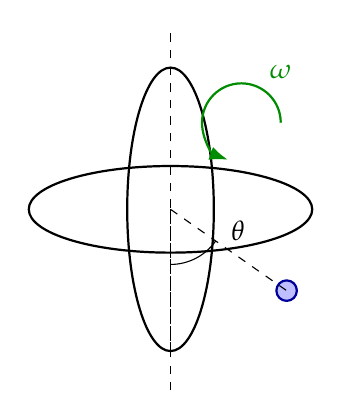
\begin{tikzpicture}[scale=1.0]
    % Lodret akse
    \draw[dashed] (0,-2.3) -- (0,2.3);
    % Ringen (set i perspektiv som ellipse)
    \draw[thick] (0,0) ellipse (1.8 and 0.55);
    \draw[thick,rotate around={90:(0,0)}] (0,0) ellipse (1.8 and 0.55);
    % Perlen
    \pgfmathsetmacro{\thetadeg}{55}
    \coordinate (B) at ({1.8*sin(\thetadeg)},{-1.8*cos(\thetadeg)});
    \filldraw[fill=blue!25,draw=blue!60!black,thick] (B) circle (0.13);
    % Vinkel theta fra bund
    \draw[dashed] (0,0) -- (0,-1.8);
    \draw[dashed] (0,0) -- (B);
    \draw (0,-0.7) arc ({-90+0}:{-90+\thetadeg}:0.7);
    \node at ({0.9*sin(\thetadeg/2+45)},{-0.9*cos(\thetadeg/2+45)}) {$\theta$};
    % Rotationspil for ringen om lodret akse
    \draw[-{Latex},thick,green!55!black] (1.4,1.1) arc (0:250:0.5);
    \node[green!55!black] at (1.4,1.75) {$\omega$};
  \end{tikzpicture}
  \caption{Perle (blå) på en cirkulær ring, der roterer med konstant
  vinkelhastighed $\omega$ om den lodrette akse. Perlens eneste
  frihedsgrad er vinklen $\theta$ målt fra ringens laveste punkt.}
  \label{fig:roterende-ring}
\end{figure}

\section{Hamiltons princip: et variationssyn}
\label{sec:hamiltons-princip}

Vi udleder nu Euler-Lagrange-ligningerne \eqref{eq:euler-lagrange} en
anden vej — ikke fra D'Alemberts differentielle princip, men fra et
globalt \emph{variationsprincip}, i tråd med udblikket i slutningen af
kapitel~\ref{kap:newton-variation}.

\subsection{Virkningen som funktional}

Betragt en tænkt bane $q_i(t)$ mellem to fastholdte tidspunkter $t_1$
og $t_2$, med fastholdte endepunkter
$q_i(t_1)=q_i^{(1)}$ og $q_i(t_2)=q_i^{(2)}$. For hver sådan bane
definerer vi \emph{virkningen}\index{virkning (Hamiltons principfunktion)}
\begin{equation}
  S[q] \equiv \int_{t_1}^{t_2} L(q(t),\dot q(t),t)\,dt.
  \label{eq:virkning}
\end{equation}
$S$ er en \emph{funktional}\index{funktional}: den tager en hel funktion $q(t)$ som
input og giver et enkelt tal som output — i modsætning til en
almindelig funktion, der tager et tal og giver et tal.
\emph{Hamiltons princip} siger:

\begin{center}
\emph{Den faktiske bane, systemet følger, er den bane, der gør $S$
\textbf{stationær} i forhold til alle nærliggende baner med samme
fastholdte endepunkter.}
\end{center}

``Stationær'' betyder her det direkte analogon til, at den afledte er
nul ved et ekstremum for en almindelig funktion — men nu i
funktionalers verden.

\subsection{Variation af virkningen}

Lad $q_i(t)$ være den (endnu ukendte) faktiske bane, og betragt en
nærliggende, tænkt bane
\begin{equation}
  \tilde q_i(t) = q_i(t) + \delta q_i(t),
\end{equation}
hvor $\delta q_i(t)$ er en arbitrær, lille afvigelsesfunktion, som
opfylder $\delta q_i(t_1)=\delta q_i(t_2)=0$ (endepunkterne er
fastholdt). Ændringen i virkningen til første orden i $\delta q_i$ er
\begin{equation}
  \delta S = \int_{t_1}^{t_2}\sum_i\left(\pdv{L}{q_i}\delta q_i + \pdv{L}{\dot q_i}\delta\dot q_i\right)dt,
\end{equation}
hvor $\delta\dot q_i = \dv*{}{t}\delta q_i$, fordi variation og
tidsafledning kommuterer (begge er blot grænseværdier af
differenskvotienter, og grænseovergangene kan ombyttes for glatte
funktioner). Vi integrerer det andet led partielt:
\begin{equation}
  \int_{t_1}^{t_2}\pdv{L}{\dot q_i}\dv{}{t}(\delta q_i)\,dt
  = \left[\pdv{L}{\dot q_i}\delta q_i\right]_{t_1}^{t_2}
    - \int_{t_1}^{t_2}\dv{}{t}\left(\pdv{L}{\dot q_i}\right)\delta q_i\,dt.
\end{equation}
Randtermen forsvinder, netop fordi $\delta q_i(t_1)=\delta q_i(t_2)=0$.
Vi står tilbage med
\begin{equation}
  \delta S = \int_{t_1}^{t_2}\sum_i\left[\pdv{L}{q_i} - \dv{}{t}\left(\pdv{L}{\dot q_i}\right)\right]\delta q_i\,dt.
  \label{eq:delta-S}
\end{equation}

\subsection{Variationsregningens grundlemma}

For at $\delta S=0$ skal gælde for \emph{enhver} tilladt afvigelse
$\delta q_i(t)$ (med de nævnte randbetingelser), må hver
koefficientfunktion i integranden være identisk nul. Dette følger af
\emph{variationsregningens fundamentallemma}: hvis en kontinuert
funktion $f(t)$ opfylder $\int_{t_1}^{t_2}f(t)\,\eta(t)\,dt=0$ for
\emph{alle} glatte $\eta(t)$ med $\eta(t_1)=\eta(t_2)=0$, så er
$f(t)\equiv 0$ på hele intervallet. (Beviset er enkelt: var $f(t_0)\neq0$
for et $t_0$ i det indre af intervallet, kunne man vælge et $\eta$, der
er positivt og koncentreret i en lille omegn om $t_0$ og nul udenfor —
og integralet ville da have samme tegn som $f(t_0)$, i modstrid med at
det skal være nul for alle $\eta$.)

Anvendt på \eqref{eq:delta-S}, koordinat for koordinat, giver dette
netop
\begin{equation}
  \dv{t}\pdv{L}{\dot q_i} - \pdv{L}{q_i} = 0, \qquad i=1,\dots,n,
\end{equation}
altså \emph{samme} Euler-Lagrange-ligninger \eqref{eq:euler-lagrange}
som i afsnit~\ref{sec:el-fra-dalembert} — nu udledt fra et rent
variationsprincip om hele banen, uden nogen reference til kræfter,
tvangskræfter eller virtuelle forskydninger ved et enkelt tidspunkt.

\begin{bemaerkning}
Det er denne ækvivalens, der gør Lagrange-formalismen så kraftfuld.
Vi har to fuldstændigt forskellige fysiske billeder — ``kræfterne
balancerer på hvert øjeblik'' (D'Alembert) og ``naturen vælger den bane,
der gør virkningen stationær'' (Hamilton) — der viser sig at give
\emph{identisk} matematisk indhold. Det er Hamiltons princip, ikke
D'Alemberts, der generaliserer til feltteori
(kapitel~\ref{kap:felter}) og til kvantemekanikkens
sti-integral-formulering, fordi det fra starten er formuleret som et
udsagn om en hel bane/historie snarere end om kræfter ved et punkt.
\end{bemaerkning}

\section{Tvangsbetingelser og Lagrange-multiplikatorer}

Indtil nu har vi forudsat, at tvangsbetingelserne allerede er
elimineret ved valg af generaliserede koordinater. Nogle gange er det
imidlertid nyttigt — eller nødvendigt, hvis man rent faktisk vil vide,
hvor stor en tvangskraft er (fx spændingen i en snor) — at beholde
flere koordinater end frihedsgrader og indføre tvangsbetingelserne
eksplicit.

Antag, at der er $m$ holonome tvangsbetingelser på formen
$f_k(q_1,\dots,q_N,t)=0$, $k=1,\dots,m$, blandt $N$ koordinater (hvor
$N>n=N-m$ er det faktiske antal frihedsgrader). Man kan da vise — ved
en variation af virkningen, hvor $\delta q_j$ nu er bundet af
$\sum_j (\partial f_k/\partial q_j)\delta q_j = 0$ for hvert $k$, og ved
at indføre Lagrange-multiplikatorer\index{Lagrange-multiplikatorer} $\lambda_k(t)$ til at håndtere
disse bindinger — at de udvidede Euler-Lagrange-ligninger bliver
\begin{equation}
  \dv{t}\pdv{L}{\dot q_j} - \pdv{L}{q_j} = \sum_{k=1}^m \lambda_k\,\pdv{f_k}{q_j}, \qquad j=1,\dots,N.
  \label{eq:el-multiplikator}
\end{equation}
De $m$ led på højresiden er netop de generaliserede tvangskræfter,
udtrykt via multiplikatorerne $\lambda_k$ — som selv bestemmes ved at
løse \eqref{eq:el-multiplikator} sammen med tvangsligningerne
$f_k=0$. Denne metode er praktisk, netop når man \emph{vil} kende
tvangskraftens størrelse (fx spændingen $\lambda$ i en snor), men vi
vil i resten af kompendiet næsten altid vælge koordinater, der
eliminerer tvangsbetingelserne fra start, som i
afsnit~\ref{sec:el-fra-dalembert}.

\section{Symmetrier og bevarelseslove: Noethers sætning}

Vi slutter kapitlet med et resultat, der viser Lagrange-formalismens
fulde styrke, og som bliver central senere i kompendiet: forbindelsen
mellem \emph{symmetrier} i $L$ og \emph{bevarelseslove}.

\subsection{Cykliske koordinater}

Antag, at $L$ ikke afhænger af en bestemt koordinat $q_k$ — dvs.
$\partial L/\partial q_k = 0$, selvom $L$ udmærket kan afhænge af
$\dot q_k$. En sådan koordinat kaldes \emph{cyklisk}\index{cyklisk koordinat}. Euler-Lagrange-
ligningen for $q_k$ reduceres da til
\begin{equation}
  \dv{t}\pdv{L}{\dot q_k} = 0
  \quad\Longrightarrow\quad
  p_k \equiv \pdv{L}{\dot q_k} = \text{konstant}.
  \label{eq:cyklisk-bevarelse}
\end{equation}
Størrelsen $p_k$ kaldes den \emph{generaliserede (kanoniske)
impuls}\index{kanonisk impuls}
konjugeret til $q_k$, og vi ser her det første eksempel på et
gennemgående mønster: \emph{en kontinuert symmetri i $L$ (uafhængighed
af en koordinat) giver en bevaret størrelse}. Vi vil møde $p_k$ igen
som en central variabel, når vi går videre til Hamilton-formalismen i
kapitel~\ref{kap:hamilton}.

\begin{eksempel}
For en fri partikel i et plan, $L=\frac12 m(\dot x^2+\dot y^2)$, er
både $x$ og $y$ cykliske. De bevarede impulser er
$p_x=m\dot x$ og $p_y=m\dot y$ — de sædvanlige kartesiske
bevægelsesmængder. For en central kraft i planpolar-koordinater,
$L=\frac12 m(\dot r^2+r^2\dot\phi^2)-V(r)$, er $\phi$ cyklisk (fordi
$V$ kun afhænger af $r$), og den bevarede størrelse er
$p_\phi=mr^2\dot\phi$ — det \emph{arealhastighedsmoment}, vi kender fra
Keplers anden lov.
\end{eksempel}

\subsection{Noethers sætning (translationssymmetri i tid)}

Cyklicitet er et specialtilfælde af en mere generel sætning, formuleret
af Emmy Noether\index{Noethers sætning}: \emph{til hver kontinuert symmetri af virkningen svarer
en bevaret størrelse}. Vi viser her det simpleste og for vores formål
vigtigste eksempel: symmetri under tidstranslation, som giver
energibevarelse.

Antag, at $L$ ikke afhænger eksplicit af $t$: $\partial L/\partial t=0$
(systemet er ``tidsinvariant'' — de fysiske love, det følger, ændrer sig
ikke fra et tidspunkt til et andet). Vi beregner den totale tidsafledte
af $L$ langs en faktisk løsning $q_i(t)$:
\begin{equation}
  \dv{L}{t} = \sum_i\left(\pdv{L}{q_i}\dot q_i + \pdv{L}{\dot q_i}\ddot q_i\right) + \pdv{L}{t}.
\end{equation}
Da $\partial L/\partial t=0$ per antagelse, og da vi langs en faktisk
løsning kan bruge Euler-Lagrange-ligningen
$\partial L/\partial q_i = \dv*{}{t}(\partial L/\partial \dot q_i)$ til
at omskrive det første led:
\begin{equation}
  \dv{L}{t} = \sum_i\left[\dv{}{t}\left(\pdv{L}{\dot q_i}\right)\dot q_i + \pdv{L}{\dot q_i}\ddot q_i\right]
  = \dv{}{t}\sum_i \dot q_i\pdv{L}{\dot q_i},
\end{equation}
hvor sidste skridt er produktreglen læst baglæns. Vi kan derfor skrive
\begin{equation}
  \dv{}{t}\left(\sum_i \dot q_i\pdv{L}{\dot q_i} - L\right) = 0,
\end{equation}
altså er størrelsen
\begin{equation}
  \boxed{H \equiv \sum_i \dot q_i\pdv{L}{\dot q_i} - L}
  \label{eq:def-H-forlobig}
\end{equation}
bevaret, når $L$ ikke afhænger eksplicit af tiden. Denne størrelse
kalder vi $H$ — og notationen er ikke tilfældig: dette er præcis den
kombination, der bliver til \emph{Hamilton-funktionen}, når vi i
kapitel~\ref{kap:hamilton} genindfører den systematisk via en
Legendre-transformation af $L$. For de fleste systemer, vi møder her —
hvor tvangsbetingelserne er tidsuafhængige, og $V$ ikke afhænger af
hastigheder — falder $H$ sammen med den samlede mekaniske energi
$T+V$, men vi udskyder det fulde bevis og den generelle diskussion
(inklusive tilfælde, hvor de \emph{ikke} falder sammen) til
kapitel~\ref{kap:hamilton}.

\begin{bemaerkning}
Vi har her set to eksempler på samme mønster: uafhængighed af $q_k$
(rumlig symmetri i en koordinat) giver bevaret impuls $p_k$;
uafhængighed af $t$ (tidssymmetri) giver bevaret ``energi'' $H$. Dette er
ikke en tilfældighed, men et specialtilfælde af Noethers generelle
sætning, som forbinder \emph{enhver} kontinuert symmetri af $L$ (under
en familie af transformationer parametriseret af én reel parameter)
med en tilsvarende bevaret størrelse. Den fulde, generelle formulering
af Noethers sætning — for en vilkårlig kontinuert transformation af
$q_i$ og $t$ — er ikke nødvendig for vores formål her, men mønstret
``symmetri $\leftrightarrow$ bevarelseslov'' vender vi tilbage til i
kapitel~\ref{kap:felter}, hvor det bliver et af de bærende principper
for klassisk feltteori.
\end{bemaerkning}

\section{Opsummering}

\begin{itemize}
  \item Ved at udtrykke D'Alemberts princip i generaliserede
        koordinater — hvor $\delta q_i$ er uafhængige — fås
        Euler-Lagrange-ligningerne
        $\dv*{}{t}(\partial L/\partial\dot q_i) - \partial L/\partial q_i = 0$,
        med $L=T-V$.
  \item Samme ligninger følger fra Hamiltons princip: den faktiske bane
        gør virkningen $S=\int L\,dt$ stationær blandt alle baner med
        fastholdte endepunkter. De to udledninger er ækvivalente, men
        det er variationssynet (Hamiltons princip), der generaliserer
        til feltteori og kvantemekanik.
  \item Tvangsbetingelser, man ikke ønsker at eliminere ved
        koordinatvalg, kan håndteres med Lagrange-multiplikatorer,
        som samtidig giver tvangskraftens størrelse.
  \item En cyklisk koordinat ($\partial L/\partial q_k=0$) giver en
        bevaret generaliseret impuls $p_k=\partial L/\partial\dot q_k$.
        Tidsuafhængighed af $L$ giver på samme måde en bevaret
        størrelse $H=\sum_i\dot q_i(\partial L/\partial\dot q_i)-L$ —
        et forvarsel om Hamilton-funktionen i
        kapitel~\ref{kap:hamilton}.
\end{itemize}

\begin{opgave}
Gennemfør selv den udregning af $T=\frac12 m(\dot x^2+\dot y^2+\dot z^2)$,
der blev sprunget over i eksemplet med den roterende ring, og
bekræft resultatet $T=\frac12 mR^2\dot\theta^2+\frac12 mR^2\omega^2\sin^2\theta$.
\end{opgave}

\begin{opgave}
En partikel med masse $m$ bevæger sig i planet under indflydelse af en
central kraft med potential $V(r)$. Opskriv Lagrange-funktionen i
planpolar-koordinater $(r,\phi)$, vis at $\phi$ er cyklisk, og udled
bevægelsesligningen for $r(t)$ ved brug af den bevarede impuls
$p_\phi=mr^2\dot\phi$ til at eliminere $\dot\phi$. Sammenlign med det
velkendte ``effektive potential'' $V_\text{eff}(r)=V(r)+p_\phi^2/(2mr^2)$.
\end{opgave}

\begin{opgave}
Vis, at for et system, hvor $\vb{r}_\alpha$ ikke afhænger eksplicit af
tiden (tidsuafhængige tvangsbetingelser, så $\partial\vb{r}_\alpha/\partial t=0$)
og hvor $V$ ikke afhænger af hastigheder, er $T$ en homogen
andengradsfunktion af $\dot q_i$, og brug Eulers sætning om homogene
funktioner ($\sum_i \dot q_i\,\partial T/\partial \dot q_i = 2T$) til at
vise, at $H$ defineret i \eqref{eq:def-H-forlobig} netop reducerer til
$H=T+V$ i dette tilfælde.
\end{opgave}

% kap03.tex — Hamilton-formalisme
% Hamilton-Jacobi-kompendiet

\chapter{Hamilton-formalisme}
\label{kap:hamilton}

\section{Målet: fra hastigheder til impulser}

I kapitel~\ref{kap:lagrange} stødte vi to gange på den generaliserede
impuls $p_i=\partial L/\partial\dot q_i$ (afsnit om cykliske
koordinater) og på størrelsen
$H=\sum_i\dot q_i\,\partial L/\partial\dot q_i - L$
(afsnit om Noethers sætning), uden at give dem en systematisk
behandling. I dette kapitel gør vi netop det: vi bytter de $n$
generaliserede hastigheder $\dot q_i$ ud med de $n$ generaliserede
impulser $p_i$ som de fundamentale variable, og omskriver hele
dynamikken i termer af $(q_i,p_i)$ i stedet for $(q_i,\dot q_i)$.

Det matematiske redskab til denne ombytning er
\emph{Legendre-transformationen}\index{Legendre-transformation}. Resultatet er \emph{Hamiltons
ligninger}\index{Hamiltons ligninger} — to \emph{første}ordens differentialligninger for hver
frihedsgrad, i stedet for Euler-Lagranges \emph{ene anden}ordens
ligning. Denne omskrivning er ikke blot kosmetisk: den flytter
beskrivelsen fra konfigurationsrummet ($n$-dimensionalt, koordinaterne
$q_i$) til \emph{faserummet}\index{faserum} ($2n$-dimensionalt, $(q_i,p_i)$), som er
selve arenaen for al den resterende teori i kompendiet — kanoniske
transformationer, Poisson-parenteser og til sidst Hamilton-Jacobi-
ligningen selv.

\section{Legendre-transformationen}

\subsection{Den generelle idé, illustreret i én variabel}

Før vi anvender Legendre-transformationen på $L$, er det nyttigt at se
den i sin enkleste form. Lad $f(x)$ være en konveks funktion af én
variabel $x$ (dvs.\ $f''(x)>0$ overalt). Vi definerer en ny variabel
\begin{equation}
  p \equiv \dv{f}{x},
\end{equation}
og — fordi $f$ er konveks, er $p(x)$ monotont voksende og dermed
invertibel: vi kan i princippet løse for $x$ som funktion af $p$. Den
\emph{Legendre-transformerede} funktion defineres som
\begin{equation}
  g(p) \equiv x\,p - f(x), \qquad \text{hvor } x = x(p) \text{ (den inverse funktion).}
  \label{eq:legendre-generel}
\end{equation}
Pointen er, at $g$ indeholder \emph{præcis} den samme information som
$f$ — vi kan altid gå tilbage — men udtrykt i den nye variabel $p$ i
stedet for $x$. At vi ganger med $p$ og trækker $f$ fra, er ikke en
arbitrær opskrift: det er netop den kombination, der garanterer, at
$dg/dp = x$ (vis selv dette ved at differentiere
\eqref{eq:legendre-generel} med hensyn til $p$ og bruge
$dp/dx\cdot dx/dp=1$), så transformationen er sin egen invers, op til
et fortegn — en symmetri, vi skal udnytte om et øjeblik.

\begin{bemaerkning}
Legendre-transformationen er langt fra unik for mekanik. Den samme
konstruktion optræder i termodynamikken (fra intern energi $U(S,V)$
til fri energi $F(T,V)=U-TS$, hvor $T=\partial U/\partial S$) og i
konveks optimering. Den fælles struktur er altid: erstat en variabel
med dens ``partielle afledte-partner'', og betal for skiftet med et
produktled.
\end{bemaerkning}

\subsection{Anvendt på Lagrange-funktionen}

Vi anvender nu \eqref{eq:legendre-generel} led for led på
$L(q_1,\dots,q_n,\dot q_1,\dots,\dot q_n,t)$, med de $n$ hastigheder
$\dot q_i$ som de variable, der skal udskiftes. For hver $i$ definerer
vi den \emph{kanoniske impuls}\index{kanonisk impuls}
\begin{equation}
  \boxed{p_i \equiv \pdv{L}{\dot q_i}.}
  \label{eq:def-p}
\end{equation}
For at denne transformation er veldefineret — dvs.\ at vi entydigt kan
løse \eqref{eq:def-p} for $\dot q_i$ som funktion af $(q,p,t)$ — skal
Hesse-matricen
\begin{equation}
  \left(\pdv[2]{L}{\dot q_i}{\dot q_j}\right)
\end{equation}
være ikke-singulær (invertibel implicit funktionssætning). Dette er
opfyldt for stort set alle fysisk relevante Lagrange-funktioner —
konkret er det opfyldt, når den kinetiske energi $T$ er en ægte
kvadratisk (positivt definit) funktion af hastighederne, hvad den er
for alle systemer, vi møder i dette kompendium.

\begin{bemaerkning}
Systemer, hvor Hesse-matricen \emph{er} singulær, kaldes
``tvangssystemer'' (constrained systems) i en teknisk betydning, der er
snævrere end de holonome tvangsbetingelser fra
kapitel~\ref{kap:newton-variation} — de kræver Diracs teori for
tvangssystemer. Dette optræder typisk for felter med gaugesymmetri
(elektromagnetisme, Yang-Mills-teori), og bliver derfor relevant, når
vi i kapitel~\ref{kap:felter} og i det senere QFT-kompendium når til
gaugefelter. Vi nævner det her, så du genkender det, når det opstår —
men det ligger uden for dette kompendiums rækkevidde at behandle det.
\end{bemaerkning}

Vi definerer nu \emph{Hamilton-funktionen}\index{Hamilton-funktion} som den
Legendre-transformerede af $L$ med hensyn til alle $\dot q_i$
samtidigt:
\begin{equation}
  \boxed{H(q,p,t) \equiv \sum_{i=1}^n p_i\dot q_i - L(q,\dot q,t),}
  \label{eq:def-H}
\end{equation}
hvor $\dot q_i$ på højresiden skal udtrykkes ved $(q,p,t)$ via den
(lokale) inversion af \eqref{eq:def-p}. Dette er netop den størrelse,
vi kaldte $H$ i \eqref{eq:def-H-forlobig} i kapitel~\ref{kap:lagrange}
— nu givet en fuldstændig, systematisk definition som funktion af
$(q,p,t)$ i stedet for $(q,\dot q,t)$.

\section{Hamiltons ligninger}

\subsection{Udledning ved direkte differentiation}

Vi differentierer definitionen \eqref{eq:def-H} totalt:
\begin{equation}
  dH = \sum_i\left(\dot q_i\,dp_i + p_i\,d\dot q_i\right) - dL.
\end{equation}
Da $L=L(q,\dot q,t)$, er
\begin{equation}
  dL = \sum_i\left(\pdv{L}{q_i}dq_i + \pdv{L}{\dot q_i}d\dot q_i\right) + \pdv{L}{t}dt
     = \sum_i\left(\pdv{L}{q_i}dq_i + p_i\,d\dot q_i\right) + \pdv{L}{t}dt,
\end{equation}
hvor vi brugte definitionen \eqref{eq:def-p} i sidste skridt. Indsat i
udtrykket for $dH$ ovenfor ser vi, at leddene med $d\dot q_i$
\emph{går ud} — det er netop pointen ved en Legendre-transformation:
\begin{equation}
  dH = \sum_i\left(\dot q_i\,dp_i - \pdv{L}{q_i}dq_i\right) - \pdv{L}{t}dt.
  \label{eq:dH-mellemresultat}
\end{equation}
Vi genkender nu $\partial L/\partial q_i$ fra Euler-Lagrange-ligningen
\eqref{eq:euler-lagrange}: langs en faktisk løsning er
$\partial L/\partial q_i = \dv*{}{t}(\partial L/\partial \dot q_i) =
\dot p_i$. Med denne substitution bliver
\eqref{eq:dH-mellemresultat}:
\begin{equation}
  dH = \sum_i\left(\dot q_i\,dp_i - \dot p_i\,dq_i\right) - \pdv{L}{t}dt.
  \label{eq:dH-slutresultat}
\end{equation}

På den anden side er $H=H(q,p,t)$ per konstruktion, så den totale
differential \emph{også} kan skrives
\begin{equation}
  dH = \sum_i\left(\pdv{H}{q_i}dq_i + \pdv{H}{p_i}dp_i\right) + \pdv{H}{t}dt.
  \label{eq:dH-fra-H}
\end{equation}
Da $q_i$, $p_i$ og $t$ er uafhængige variable i $H$'s beskrivelse, må
koefficienterne til $dq_i$, $dp_i$ og $dt$ i
\eqref{eq:dH-slutresultat} og \eqref{eq:dH-fra-H} stemme overens led
for led. Dette giver os \emph{Hamiltons ligninger}:
\begin{equation}
  \boxed{\dot q_i = \pdv{H}{p_i}, \qquad \dot p_i = -\pdv{H}{q_i}, \qquad i=1,\dots,n,}
  \label{eq:hamiltons-ligninger}
\end{equation}
samt, som en biprodukt af samme sammenligning,
\begin{equation}
  \pdv{H}{t} = -\pdv{L}{t}.
  \label{eq:dH-dt}
\end{equation}

\begin{bemaerkning}
Hamiltons ligninger \eqref{eq:hamiltons-ligninger} er $2n$ \emph{først}e-
ordens differentialligninger, mod Euler-Lagranges $n$ \emph{anden}-
ordens ligninger. Dette er ikke en tilfældig gevinst: en tilstand i
faserummet, $(q_i(t),p_i(t))$, er nu fuldstændig bestemt af sin værdi
ved \emph{ét} tidspunkt — der er ikke brug for at kende både position
\emph{og} hastighed ved starttidspunktet særskilt, fordi $p_i$ allerede
``indeholder'' den information, der før lå i $\dot q_i$. Denne
førsteordens-struktur er præcis, hvad der gør faserumsbilledet så
naturligt, og den er en direkte forløber for tilstandsbegrebet i
kvantemekanikken, hvor en tilstand (bølgefunktionen) også er
fuldstændigt bestemt ved et enkelt tidspunkt.
\end{bemaerkning}

\subsection{Fortolkningen af $H$: bevarelse og energi}

Vi genbesøger nu \eqref{eq:dH-dt} i lyset af Hamiltons ligninger. Den
totale tidsafledte af $H$ langs en faktisk bane er
\begin{equation}
  \dv{H}{t} = \sum_i\left(\pdv{H}{q_i}\dot q_i + \pdv{H}{p_i}\dot p_i\right) + \pdv{H}{t}
  = \sum_i\left(\pdv{H}{q_i}\pdv{H}{p_i} - \pdv{H}{p_i}\pdv{H}{q_i}\right) + \pdv{H}{t}
  = \pdv{H}{t},
\end{equation}
hvor vi brugte Hamiltons ligninger \eqref{eq:hamiltons-ligninger} til
at indsætte $\dot q_i$ og $\dot p_i$, og de to led i parentesen
ophæver hinanden identisk. Vi har altså det generelle resultat
\begin{equation}
  \dv{H}{t} = \pdv{H}{t}.
  \label{eq:dHdt-generel}
\end{equation}
Specielt: hvis $H$ ikke afhænger \emph{eksplicit} af tiden
($\partial H/\partial t=0$, hvilket ifølge \eqref{eq:dH-dt} er
ækvivalent med $\partial L/\partial t=0$), er $H$ en \emph{bevaret
størrelse} langs bevægelsen — vi genfinder Noether-resultatet fra
kapitel~\ref{kap:lagrange}, nu udledt direkte i Hamilton-billedet, uden
omvejen over $L$.

For de systemer, vi typisk møder — tidsuafhængige holonome
tvangsbetingelser, og et potential $V$, der ikke afhænger af
hastigheder — viste opgave 3 i kapitel~\ref{kap:lagrange}, at
$H=T+V$, den samlede mekaniske energi. I disse tilfælde er Hamiltons
ligninger derfor blot en omskrivning af energibevarelse og
bevægelsesligningerne i førsteordensform — men formalismens virkelige
styrke viser sig, når $H\neq T+V$ (fx i tidsafhængige eller
elektromagnetiske systemer), hvor $H$ stadig er den korrekte
``generator'' af tidsudviklingen, selv om den ikke er den mekaniske
energi.

\section{Eksempel: den harmoniske oscillator i faserum}

\begin{eksempel}
For en énddimensional harmonisk oscillator med masse $m$ og
fjederkonstant $k$ er
\begin{equation}
  L = \frac12 m\dot x^2 - \frac12 kx^2.
\end{equation}
Den kanoniske impuls er
\begin{equation}
  p = \pdv{L}{\dot x} = m\dot x
  \quad\Longrightarrow\quad
  \dot x = \frac{p}{m},
\end{equation}
som her simpelthen er den velkendte bevægelsesmængde — Legendre-
transformationen er triviel at invertere for dette system. Hamilton-
funktionen bliver
\begin{equation}
  H = p\dot x - L = p\cdot\frac{p}{m} - \left(\frac12 m\left(\frac{p}{m}\right)^2 - \frac12 kx^2\right)
    = \frac{p^2}{2m} + \frac12 kx^2,
\end{equation}
altså netop $T+V$ udtrykt ved $p$ i stedet for $\dot x$, som forventet.
Hamiltons ligninger \eqref{eq:hamiltons-ligninger} giver
\begin{equation}
  \dot x = \pdv{H}{p} = \frac{p}{m}, \qquad
  \dot p = -\pdv{H}{x} = -kx.
\end{equation}
Den første ligning er blot definitionen af $p$ igen (som det altid vil
være for et system uden hastighedsafhængigt potential); den anden er
Newtons anden lov, $m\ddot x=-kx$, skrevet i førsteordensform. Løsningen
er velkendt, $x(t)=A\cos(\Omega t+\varphi)$ med $\Omega=\sqrt{k/m}$, og
banen i faserummet $(x,p)$ er ellipsen
\begin{equation}
  \frac{p^2}{2mH} + \frac{x^2}{2H/k} = 1,
\end{equation}
fordi $H$ er konstant langs banen (se figur~\ref{fig:faseportraet}).
Dette er vores første eksempel på et \emph{faseportræt}\index{faseportræt}: en geometrisk
repræsentation af systemets dynamik som en kurve (eller familie af
kurver, for forskellige energier $H$) i faserummet, uden nogen
eksplicit reference til tiden $t$.
\end{eksempel}

\begin{figure}[htbp]
  \centering
  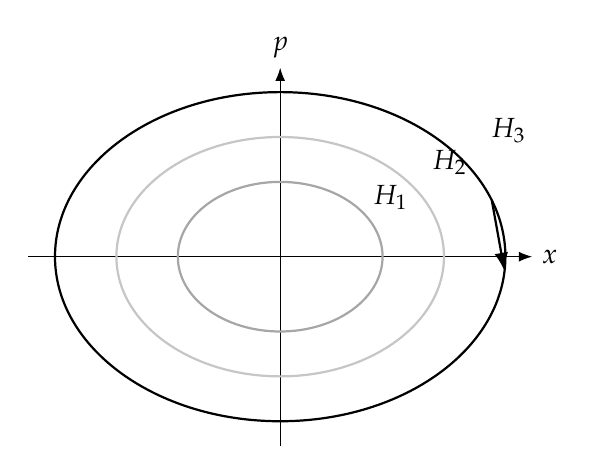
\begin{tikzpicture}[scale=1.0]
    % Akser
    \draw[-{Latex}] (-3.2,0) -- (3.2,0) node[right] {$x$};
    \draw[-{Latex}] (0,-2.4) -- (0,2.4) node[above] {$p$};
    % Familie af faseportræt-ellipser for forskellige energier
    \foreach \sc/\col in {0.5/gray!70,0.8/gray!45,1.1/black} {
      \draw[thick,\col] (0,0) ellipse ({2.6*\sc} and {1.9*\sc});
    }
    % Pil der viser bevægelsesretning (med uret) på yderste ellipse
    \draw[-{Latex},thick] ({2.6*1.1*cos(20)},{1.9*1.1*sin(20)}) -- ({2.6*1.1*cos(-5)},{1.9*1.1*sin(-5)});
    \node at (2.9,1.6) {$H_3$};
    \node at (2.15,1.2) {$H_2$};
    \node at (1.4,0.75) {$H_1$};
  \end{tikzpicture}
  \caption{Faseportræt for den harmoniske oscillator: hver ellipse er en
  bane med konstant energi $H$ (voksende fra $H_1$ til $H_3$).
  Bevægelsen langs hver ellipse sker med uret, som markeret med pilen.
  Faserumsbeskrivelsen erstatter tidsforløbet $x(t)$ med en statisk,
  geometrisk figur.}
  \label{fig:faseportraet}
\end{figure}

\section{Faserummet som arena}

Det er værd at fremhæve, hvad vi har vundet ved skiftet til
$(q_i,p_i)$. I konfigurationsrummet ($q_i$ alene) skærer baner for
forskellige startbetingelser hinanden hele tiden — en partikel, der
passerer gennem et bestemt punkt $x_0$, kan have en hvilken som helst
hastighed, så uendeligt mange baner går gennem samme punkt. I
\emph{faserummet} $(q_i,p_i)$ er dette udelukket: gennem hvert punkt
$(q_0,p_0)$ går \'en og kun \'en bane, fordi $(q_0,p_0)$ er en
fuldstændig starttilstand. Faserumsbaner for forskellige startbetingelser
kan derfor aldrig skære hinanden (bortset fra i entydige ligevægtspunkter)
— en egenskab, der bliver central, når vi i kapitel~\ref{kap:kanoniske-transf}
og \ref{kap:hj} studerer, hvordan hele familier af baner transformerer
sig samtidigt under kanoniske transformationer.

\begin{bemaerkning}
Faserummets rolle som en arena, hvori ``tilstanden'' er et punkt, og hvor
baner ikke skærer hinanden, er selve det billede, der (i en passende
kvantiseret og ``udtværet'' form, jf.\ Heisenbergs
usikkerhedsrelation) bliver til kvantemekanikkens tilstandsrum. Vejen
fra det klassiske faserum til kvantemekanikkens Hilbert-rum går netop
via de strukturer, vi udvikler i de kommende kapitler — Poisson-
parenteser (kapitel~\ref{kap:poisson}), som bliver til kommutatorer ved
kanonisk kvantisering, og Hamilton-Jacobi-ligningen
(kapitel~\ref{kap:hj}), som viser sig at være den klassiske grænse af
Schrödinger-ligningen (se [[kvantemekanik-kompendiet]] for den
kvantemekaniske side af denne forbindelse).
\end{bemaerkning}

\section{Opsummering}

\begin{itemize}
  \item Legendre-transformationen udskifter en variabel med dens
        partielle afledte-partner: $g(p)=xp-f(x)$, hvor $p=df/dx$.
  \item Anvendt på $L(q,\dot q,t)$ med $p_i=\partial L/\partial\dot q_i$
        giver dette Hamilton-funktionen
        $H(q,p,t)=\sum_i p_i\dot q_i - L$.
  \item Sammenligning af $dH$ udledt af definitionen med $dH$ udledt af
        $H(q,p,t)$ giver Hamiltons ligninger,
        $\dot q_i=\partial H/\partial p_i$,
        $\dot p_i=-\partial H/\partial q_i$ — $2n$
        førsteordensligninger i stedet for $n$ andenordensligninger.
  \item $dH/dt = \partial H/\partial t$: $H$ er bevaret, når den ikke
        afhænger eksplicit af tiden. For tidsuafhængige,
        hastighedsuafhængige potentialer er $H=T+V$.
  \item Faserummet $(q_i,p_i)$ er arenaen for resten af kompendiet:
        hvert punkt er en fuldstændig tilstand, og baner for forskellige
        starttilstande skærer aldrig hinanden.
\end{itemize}

\begin{opgave}
Opskriv Lagrange-funktionen for en partikel med masse $m$ i et
centralt potential $V(r)$ i planpolar-koordinater $(r,\phi)$ (jf.\
opgave 2 i kapitel~\ref{kap:lagrange}), udfør Legendre-transformationen
til $(p_r,p_\phi)$, og vis at
\begin{equation}
  H = \frac{p_r^2}{2m} + \frac{p_\phi^2}{2mr^2} + V(r).
\end{equation}
Opskriv Hamiltons ligninger for $(r,p_r,\phi,p_\phi)$ og sammenlign med
resultatet fra kapitel~\ref{kap:lagrange}.
\end{opgave}

\begin{opgave}
En ladet partikel med masse $m$ og ladning $e$ bevæger sig i et
elektromagnetisk felt beskrevet ved skalarpotentialet $\Phi$ og
vektorpotentialet $\vb{A}$. Lagrange-funktionen er (uden bevis her —
den udledes korrekt først i forbindelse med feltteorien i
kapitel~\ref{kap:felter})
\begin{equation}
  L = \frac12 m\dot{\vb{r}}^2 - e\Phi + e\,\dot{\vb{r}}\cdot\vb{A}.
\end{equation}
Vis, at den kanoniske impuls er $\vb{p}=m\dot{\vb{r}}+e\vb{A}$ — altså
\emph{ikke} lig med den mekaniske bevægelsesmængde $m\dot{\vb{r}}$ —
og find Hamilton-funktionen $H(\vb{r},\vb{p},t)$. Dette er det
kanoniske eksempel på, at $H$ og den mekaniske energi $T+V$ kan være to
forskellige størrelser.
\end{opgave}

\begin{opgave}
Skitser (i hånden eller med et plot) faseportrættet for en partikel med
energi $E$, der bevæger sig i et énddimensionalt potential med en
enkelt potentialbrønd (fx $V(x)=\frac12 kx^2$ for $|x|<a$ og
$V(x)=\infty$ for $|x|\geq a$, en ``boks med fjederbund''). Angiv, hvilke
værdier af $E$ der giver lukkede (periodiske) baner, og diskuter, hvad
der sker med faseportrættet, når $E$ nærmer sig den energi, hvor
partiklen netop når randen $|x|=a$.
\end{opgave}

% kap04.tex — Poisson-parenteser og kanonisk struktur
% Hamilton-Jacobi-kompendiet

\chapter{Poisson-parenteser og kanonisk struktur}
\label{kap:poisson}

\section{Tidsudviklingen af en vilkårlig størrelse}

I kapitel~\ref{kap:hamilton} udledte vi, at $dH/dt=\partial H/\partial t$
langs en faktisk bane. Det naturlige næste spørgsmål er: hvad gælder
for tidsafledningen af en \emph{vilkårlig} funktion
$f(q,p,t)$ af faserumsvariablene — ikke kun $H$ selv? Svaret på dette
spørgsmål fører os til at indføre \emph{Poisson-parentesen}\index{Poisson-parentes}, som
bliver det centrale algebraiske redskab for resten af kompendiet, og
som — det skal siges allerede her — er den klassiske forløber for
kommutatoren i kvantemekanikken.

Ved kædereglen og Hamiltons ligninger \eqref{eq:hamiltons-ligninger}:
\begin{equation}
  \dv{f}{t} = \sum_i\left(\pdv{f}{q_i}\dot q_i + \pdv{f}{p_i}\dot p_i\right) + \pdv{f}{t}
  = \sum_i\left(\pdv{f}{q_i}\pdv{H}{p_i} - \pdv{f}{p_i}\pdv{H}{q_i}\right) + \pdv{f}{t}.
  \label{eq:df-dt-udledning}
\end{equation}
Summen på højresiden — uden $\partial f/\partial t$-leddet — optræder
så ofte og med en så bestemt algebraisk struktur, at den fortjener sit
eget symbol og navn.

\section{Definition af Poisson-parentesen}

For to funktioner $f(q,p,t)$ og $g(q,p,t)$ på faserummet defineres
\emph{Poisson-parentesen}
\begin{equation}
  \boxed{\{f,g\} \equiv \sum_{i=1}^n\left(\pdv{f}{q_i}\pdv{g}{p_i} - \pdv{f}{p_i}\pdv{g}{q_i}\right).}
  \label{eq:def-poisson}
\end{equation}
Med denne definition bliver \eqref{eq:df-dt-udledning} til den
kompakte og centrale formel
\begin{equation}
  \boxed{\dv{f}{t} = \{f,H\} + \pdv{f}{t}.}
  \label{eq:bevaegelse-poisson}
\end{equation}
Dette er \emph{bevægelsesligningen for en vilkårlig faserumsfunktion},
udtrykt via Poisson-parentesen med $H$. Vi kan endda genskrive
Hamiltons ligninger selv i denne form: sæt $f=q_i$ og $f=p_i$
(begge er trivielt tidsuafhængige som funktioner, $\partial q_i/\partial t=0$),
og brug definitionen \eqref{eq:def-poisson} direkte:
\begin{equation}
  \dot q_i = \{q_i,H\} = \pdv{H}{p_i}, \qquad
  \dot p_i = \{p_i,H\} = -\pdv{H}{q_i},
\end{equation}
i fuld overensstemmelse med \eqref{eq:hamiltons-ligninger}. Hamiltons
ligninger er altså blot specialtilfælde af den generelle formel
\eqref{eq:bevaegelse-poisson}.

\section{De fundamentale parenteser}

Ved direkte indsættelse i \eqref{eq:def-poisson}, med $q_i$ og $p_i$
som de indsatte funktioner, og med Kronecker-deltaet
$\delta_{ij}=1$ for $i=j$ og $0$ ellers (fordi $\partial q_i/\partial q_j=\delta_{ij}$
og $\partial p_i/\partial p_j=\delta_{ij}$, mens $q_i$ og $p_j$ er
uafhængige, så $\partial q_i/\partial p_j=0$), finder man
\begin{equation}
  \boxed{\{q_i,q_j\} = 0, \qquad \{p_i,p_j\} = 0, \qquad \{q_i,p_j\} = \delta_{ij}.}
  \label{eq:fundamentale-parenteser}
\end{equation}
Disse tre relationer kaldes de \emph{fundamentale
Poisson-parenteser}\index{Poisson-parentes!fundamentale}.
De er selve definitionen af, hvad det betyder for et sæt variable
$(q_i,p_i)$ at være \emph{kanonisk konjugerede}\index{kanonisk konjugerede variable} — en egenskab, vi
udnytter systematisk, når vi i kapitel~\ref{kap:kanoniske-transf}
spørger, hvilke koordinatskift på faserummet bevarer Hamiltons
ligningers form.

\begin{bemaerkning}
Relationen $\{q_i,p_j\}=\delta_{ij}$ er den klassiske forgænger til
kommutationsrelationen $[\hat q_i,\hat p_j]=i\hbar\,\delta_{ij}$ i
kvantemekanikken (se [[kvantemekanik-kompendiet]]). Reglen for at gå
fra klassisk til kvantemekanik — \emph{kanonisk kvantisering} — er
netop at erstatte Poisson-parenteser med kommutatorer efter reglen
$\{f,g\}\to \frac{1}{i\hbar}[\hat f,\hat g]$. Vi vil ikke udføre
denne kvantisering i dette kompendium (det er det senere QFT-
kompendiums opgave at gøre det systematisk), men det er værd at bære
med sig, at hele den algebraiske struktur, vi bygger op i dette
kapitel, overlever næsten ord for ord ind i kvanteteorien.
\end{bemaerkning}

\section{Algebraiske egenskaber}

Poisson-parentesen har en række egenskaber, som gør den til en såkaldt
\emph{Lie-parentes}\index{Lie-algebra} — den samme abstrakte struktur, man møder i teorien
for kontinuerte symmetrigrupper. Vi angiver dem her; de følger alle
direkte af definitionen \eqref{eq:def-poisson} ved indsættelse (se
opgave 1).

\begin{itemize}
  \item \textbf{Antisymmetri:} $\{f,g\} = -\{g,f\}$. Specielt
        $\{f,f\}=0$.
  \item \textbf{Bilinearitet:} $\{af+bg,h\} = a\{f,h\}+b\{g,h\}$ for
        konstanter $a,b$ (og tilsvarende i det andet argument, via
        antisymmetrien).
  \item \textbf{Leibniz-regel (produktregel):}
        $\{fg,h\} = f\{g,h\} + \{f,h\}g$.
  \item \textbf{Jacobi-identiteten:}\index{Jacobi-identiteten}
        \begin{equation}
          \{f,\{g,h\}\} + \{g,\{h,f\}\} + \{h,\{f,g\}\} = 0.
        \end{equation}
\end{itemize}

Jacobi-identiteten er den mindst intuitive, men også den vigtigste af
de fire: det er den, der garanterer, at Poisson-parenteser (og senere
kommutatorer) definerer en konsistent algebraisk struktur, som man kan
bygge en gruppeteori af symmetritransformationer ovenpå.

\begin{bemaerkning}
Et sæt størrelser, der er lukket under Poisson-parentesen — dvs.\
hvor $\{f,g\}$ altid selv kan skrives som en (lineær) kombination af
størrelserne i sættet — udgør, hvad man kalder en \emph{Lie-algebra}.
Dette er præcis den struktur, der ligger bag begrebet "symmetrigruppe"
i fysikken: banemomentkomponenterne $(L_x,L_y,L_z)$, som vi ser i
næste afsnit, er det arketypiske eksempel, og deres Poisson-
algebra er den klassiske skygge af rotationsgruppens
kommutationsrelationer i kvantemekanikken.
\end{bemaerkning}

\section{Bevarelseslove via Poisson-parenteser}

Formel \eqref{eq:bevaegelse-poisson} giver et umiddelbart og meget
anvendt kriterium for bevarelse: hvis $f$ ikke afhænger eksplicit af
tiden ($\partial f/\partial t=0$), så er
\begin{equation}
  \boxed{f \text{ er bevaret} \quad\Longleftrightarrow\quad \{f,H\}=0.}
  \label{eq:bevarelse-poisson}
\end{equation}
Dette generaliserer både resultatet for cykliske koordinater
(kapitel~\ref{kap:lagrange}) og for $H$ selv
(kapitel~\ref{kap:hamilton}, hvor $\{H,H\}=0$ trivielt pga.\
antisymmetrien, så $H$ er bevaret netop når $\partial H/\partial t=0$,
som vi allerede vidste).

\begin{bemaerkning}
Et vigtigt strukturelt resultat, som følger direkte af Jacobi-
identiteten (se opgave 2), er, at hvis $f$ og $g$ begge er bevarede
størrelser (begge Poisson-kommuterer med $H$), så er deres Poisson-
parentes $\{f,g\}$ \emph{også} en bevaret størrelse. Bevarede
størrelser er altså lukkede under Poisson-parentesen — de udgør netop
en Lie-algebra i den forstand, der blev nævnt ovenfor. Dette er
oprindelsen til, at bevægelseskonstanter for et system med
tilstrækkeligt mange symmetrier ofte "kommer i familier", der danner
en gruppe (rotationsgruppen for banemoment er det stående eksempel).
\end{bemaerkning}

\subsection{Eksempel: banemomentets Poisson-algebra}

\begin{eksempel}
Betragt banemomentets\index{banemoment} tre kartesiske komponenter for en partikel i tre
dimensioner,
\begin{equation}
  L_x = yp_z - zp_y, \qquad L_y = zp_x - xp_z, \qquad L_z = xp_y - yp_x,
\end{equation}
udtrykt ved de kanoniske variable $(x,y,z,p_x,p_y,p_z)$, som opfylder
de fundamentale parenteser \eqref{eq:fundamentale-parenteser} (med
$q_1,q_2,q_3=x,y,z$). Vi beregner $\{L_x,L_y\}$ direkte fra
definitionen \eqref{eq:def-poisson},
\begin{equation}
  \{L_x,L_y\} = \sum_{i\in\{x,y,z\}}\left(\pdv{L_x}{i}\pdv{L_y}{p_i} - \pdv{L_x}{p_i}\pdv{L_y}{i}\right),
\end{equation}
ved først at opskrive alle de nødvendige partielle afledte:
\begin{equation}
  \pdv{L_x}{x}=0,\quad \pdv{L_x}{y}=p_z,\quad \pdv{L_x}{z}=-p_y,\quad
  \pdv{L_x}{p_x}=0,\quad \pdv{L_x}{p_y}=-z,\quad \pdv{L_x}{p_z}=y,
\end{equation}
\begin{equation}
  \pdv{L_y}{x}=-p_z,\quad \pdv{L_y}{y}=0,\quad \pdv{L_y}{z}=p_x,\quad
  \pdv{L_y}{p_x}=z,\quad \pdv{L_y}{p_y}=0,\quad \pdv{L_y}{p_z}=-x.
\end{equation}
Bidraget fra $i=x$ er $\left(\partial_xL_x\right)\left(\partial_{p_x}L_y\right)-\left(\partial_{p_x}L_x\right)\left(\partial_xL_y\right)=0\cdot z-0\cdot(-p_z)=0$,
og bidraget fra $i=y$ er ligeledes $p_z\cdot 0-(-z)\cdot 0=0$: begge
forsvinder, fordi enten $L_x$ eller $L_y$ mangler den relevante
afhængighed. Kun $i=z$ bidrager:
\begin{equation}
  \left(\pdv{L_x}{z}\right)\left(\pdv{L_y}{p_z}\right) - \left(\pdv{L_x}{p_z}\right)\left(\pdv{L_y}{z}\right)
  = (-p_y)(-x) - (y)(p_x) = xp_y - yp_x = L_z.
\end{equation}
Vi finder altså
\begin{equation}
  \boxed{\{L_x,L_y\} = L_z,}
  \label{eq:Lx-Ly}
\end{equation}
og ved cyklisk ombytning af $(x,y,z)$:
\begin{equation}
  \{L_y,L_z\} = L_x, \qquad \{L_z,L_x\} = L_y.
\end{equation}
Banemomentets tre komponenter er altså \emph{lukkede} under Poisson-
parentesen — de danner en Lie-algebra, isomorf til rotationsgruppen
$SO(3)$'s Lie-algebra. Dette er den klassiske skygge af de velkendte
kommutationsrelationer $[\hat L_x,\hat L_y]=i\hbar\hat L_z$ (cyklisk) i
kvantemekanikken (se [[kvantemekanik-kompendiet]]).
\end{eksempel}

\section{Liouvilles sætning: bevarelse af faserumsvolumen}

Vi slutter kapitlet med et geometrisk resultat, der binder Poisson-
strukturen sammen med faserumsbilledet fra
kapitel~\ref{kap:hamilton}. Betragt en samling af systemer med
starttilstande fordelt over et lille område $\Omega_0$ i faserummet
(fx alle med næsten samme $(q,p)$, men med små variationer). Under
tidsudviklingen bevæger hvert punkt i $\Omega_0$ sig efter Hamiltons
ligninger, og området deformeres til et nyt område $\Omega_t$.

\emph{Liouvilles sætning}\index{Liouvilles sætning} siger, at \emph{volumenet} af dette område i
faserummet er \emph{bevaret}:
\begin{equation}
  \text{Vol}(\Omega_t) = \text{Vol}(\Omega_0) \qquad \text{for alle } t.
  \label{eq:liouville}
\end{equation}
Den underliggende grund er, at Hamiltons ligninger definerer et
"strømningsfelt" på faserummet,
$\vb{v}=(\dot q_1,\dots,\dot q_n,\dot p_1,\dots,\dot p_n)$, hvis
divergens er identisk nul:
\begin{equation}
  \sum_i\left(\pdv{\dot q_i}{q_i} + \pdv{\dot p_i}{p_i}\right)
  = \sum_i\left(\pdv{}{q_i}\pdv{H}{p_i} - \pdv{}{p_i}\pdv{H}{q_i}\right) = 0,
\end{equation}
fordi de to blandede andenafledte af $H$ er identiske og trækkes fra
hinanden. Et divergensfrit strømningsfelt bevarer volumen, ganske som
en inkompressibel væskestrømning — dette er indholdet af
\eqref{eq:liouville}.

\begin{bemaerkning}
Liouvilles sætning er grundstenen for al klassisk statistisk mekanik:
den garanterer, at en sandsynlighedsfordeling over faserummet
udvikler sig som et inkompressibelt "faserumsfluidum", hvilket er
udgangspunktet for Liouville-ligningen for fordelingsfunktionen
$\rho(q,p,t)$. Vi forfølger ikke denne retning i dette kompendium, men
den er værd at nævne, fordi den samme volumenbevarelse (nu udtrykt som
unitaritet af tidsudviklingen) er en af de mest grundlæggende
egenskaber, kvantemekanikken må arve fra den klassiske teori.
\end{bemaerkning}

\begin{figure}[htbp]
  \centering
  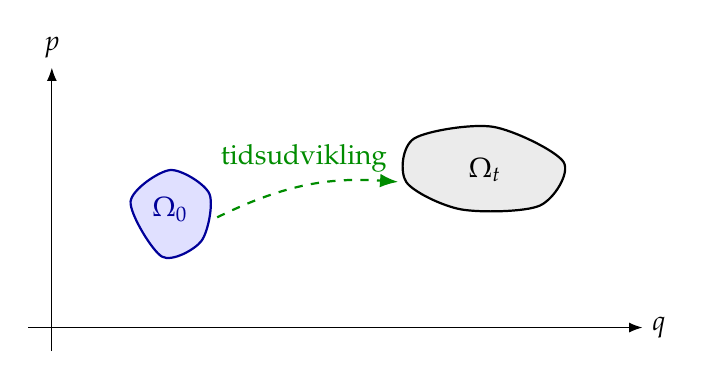
\begin{tikzpicture}[scale=1.0]
    \draw[-{Latex}] (-0.3,0) -- (7.5,0) node[right] {$q$};
    \draw[-{Latex}] (0,-0.3) -- (0,3.3) node[above] {$p$};
    % Oprindeligt område Omega_0 (cirkulær-ish blob)
    \draw[thick,blue!60!black,fill=blue!12] plot[smooth cycle] coordinates
      {(1.0,1.6) (1.5,2.0) (2.0,1.7) (1.9,1.1) (1.4,0.9)};
    \node[blue!60!black] at (1.5,1.5) {$\Omega_0$};
    % Deformeret område Omega_t (aflangt, samme areal, forskudt)
    \draw[thick,black,fill=black!8] plot[smooth cycle] coordinates
      {(4.6,2.4) (5.6,2.55) (6.5,2.1) (6.2,1.55) (5.2,1.5) (4.5,1.85)};
    \node at (5.5,2.0) {$\Omega_t$};
    % Pil der viser strømningen/tidsudviklingen
    \draw[-{Latex},thick,dashed,green!55!black] (2.1,1.4) to[bend left=15] (4.4,1.85);
    \node[green!55!black] at (3.2,2.15) {tidsudvikling};
  \end{tikzpicture}
  \caption{Liouvilles sætning: et område $\Omega_0$ i faserummet
  deformeres under tidsudviklingen til $\Omega_t$ — formen ændres,
  men arealet (i to dimensioner) hhv.\ volumenet (i $2n$ dimensioner)
  er bevaret.}
  \label{fig:liouville}
\end{figure}

\section{Opsummering}

\begin{itemize}
  \item Poisson-parentesen $\{f,g\}=\sum_i(\partial_{q_i}f\,\partial_{p_i}g - \partial_{p_i}f\,\partial_{q_i}g)$
        opsummerer tidsudviklingen af enhver faserumsfunktion:
        $df/dt = \{f,H\} + \partial f/\partial t$.
  \item De fundamentale parenteser $\{q_i,p_j\}=\delta_{ij}$,
        $\{q_i,q_j\}=\{p_i,p_j\}=0$ definerer, hvad det betyder at være
        kanonisk konjugerede variable.
  \item Poisson-parentesen er antisymmetrisk, bilineær, opfylder
        Leibniz-reglen og Jacobi-identiteten — den er en Lie-parentes.
  \item En tidsuafhængig størrelse $f$ er bevaret netop når
        $\{f,H\}=0$; bevarede størrelser er lukkede under
        Poisson-parentesen.
  \item Banemomentets komponenter opfylder $\{L_x,L_y\}=L_z$ (cyklisk)
        — den klassiske forløber for rotationsgruppens
        kommutationsrelationer.
  \item Liouvilles sætning: faserumsvolumen er bevaret under
        Hamiltons ligningers tidsudvikling, fordi strømningsfeltet er
        divergensfrit.
\end{itemize}

\begin{opgave}
Vis direkte fra definitionen \eqref{eq:def-poisson}, at Poisson-
parentesen er antisymmetrisk og opfylder Leibniz-reglen
$\{fg,h\}=f\{g,h\}+\{f,h\}g$.
\end{opgave}

\begin{opgave}
Brug Jacobi-identiteten til at vise, at hvis $\{f,H\}=0$ og
$\{g,H\}=0$ (begge tidsuafhængige og bevarede), så er
$\{\{f,g\},H\}=0$ — altså at $\{f,g\}$ også er bevaret. (Antag
$\partial f/\partial t=\partial g/\partial t=0$.)
\end{opgave}

\begin{opgave}
Gennemfør den fulde udregning af $\{L_x,L_y\}$ fra definitionen
\eqref{eq:def-poisson}, led for led, og bekræft resultatet
\eqref{eq:Lx-Ly}. Vis derudover, at $\{L_z,x\}=-y$ og $\{L_z,y\}=x$
(dvs.\ at $L_z$ genererer infinitesimale rotationer om $z$-aksen —
en forsmag på den generelle forbindelse mellem Poisson-parenteser og
symmetritransformationer, som vender tilbage i
kapitel~\ref{kap:kanoniske-transf}).
\end{opgave}

% kap05.tex — Kanoniske transformationer
% Hamilton-Jacobi-kompendiet

\chapter{Kanoniske transformationer}
\label{kap:kanoniske-transf}

\section{Motivation: frihed til at vælge faserumskoordinater}

I Lagrange-formalismen (kapitel~\ref{kap:lagrange}) kan vi vælge
generaliserede koordinater $q_i$ helt frit — enhver invertibel
omskrivning $Q_i=Q_i(q,t)$ giver stadig Euler-Lagrange-ligninger af
samme form. Spørgsmålet i dette kapitel er, om der findes en analog
frihed i Hamilton-formalismen: kan vi skifte til nye faserums\-
koordinater $(Q_i,P_i)$ — ikke kun nye $Q_i$, men også nye $P_i$, som
kan blande de gamle $q_i$ og $p_i$ på vilkårlig vis — og stadig have
Hamiltons ligninger på samme form,
\begin{equation}
  \dot Q_i = \pdv{K}{P_i}, \qquad \dot P_i = -\pdv{K}{Q_i},
  \label{eq:hamilton-nye-var}
\end{equation}
for en ny Hamilton-funktion $K(Q,P,t)$?

Svaret er ja, og mængden af sådanne transformationer er langt større
end i Lagrange-billedet — netop fordi $q_i$ og $p_i$ i Hamilton-
formalismen spiller en langt mere symmetrisk rolle end $q_i$ og
$\dot q_i$ gør i Lagrange-formalismen. Denne frihed er ikke blot en
teoretisk raffinement: det er selve kernen i strategien bag
Hamilton-Jacobi-teorien (kapitel~\ref{kap:hj}), hvor vi søger en
kanonisk transformation, der gør den \emph{nye} Hamilton-funktion
identisk nul — hvorved bevægelsesligningerne i de nye variable bliver
trivielle, $\dot Q_i=\dot P_i=0$.

\section{Definition}

En transformation $(q_i,p_i)\to(Q_i,P_i)$ (eventuelt tidsafhængig)
kaldes \emph{kanonisk}\index{kanonisk transformation}, hvis den bevarer Hamiltons ligningers form: der
findes en funktion $K(Q,P,t)$, så \eqref{eq:hamilton-nye-var} er
opfyldt for enhver Hamilton-funktion $H$, systemet kunne have. Vi skal
nu udlede en konstruktiv metode til at frembringe sådanne
transformationer — via \emph{genererende funktioner}.

\section{Det modificerede Hamiltons princip}

Hamiltons princip (afsnit~\ref{sec:hamiltons-princip}) kan omskrives i
faserumsvariable. Ved at bruge $L=\sum_i p_i\dot q_i - H$ (omskrivning
af definitionen \eqref{eq:def-H}), bliver virkningen
\begin{equation}
  S = \int_{t_1}^{t_2}\left(\sum_i p_i\dot q_i - H\right)dt,
\end{equation}
og variation af $S$ med hensyn til \emph{uafhængige} variationer i
$q_i$ og $p_i$ (ikke kun $q_i$, som i afsnit~\ref{sec:hamiltons-princip})
giver netop Hamiltons ligninger som Euler-Lagrange-ligninger for dette
udvidede variationsprincip (se opgave 1). For at de \emph{nye}
variable $(Q_i,P_i)$ skal opfylde Hamiltons ligninger med en ny
Hamilton-funktion $K$, skal det tilsvarende princip
\begin{equation}
  \delta\int_{t_1}^{t_2}\left(\sum_i P_i\dot Q_i - K\right)dt = 0
\end{equation}
gælde \emph{samtidig} med det oprindelige. Dette er sikret, hvis
integranderne kun adskiller sig ved en total tidsafledt af en funktion
$F$ — for et sådant led bidrager kun med randtermer, som ikke påvirker
variationen, når endepunkterne er fastholdt (præcis som i
udledningen af \eqref{eq:delta-S}):
\begin{equation}
  \sum_i p_i\dot q_i - H = \sum_i P_i\dot Q_i - K + \dv{F}{t}.
  \label{eq:genererende-betingelse}
\end{equation}
Funktionen $F$ kaldes den \emph{genererende funktion}\index{genererende funktion} for
transformationen. Den kan i princippet afhænge af en blanding af
gamle og nye variable — det er netop valget af, hvilke variable $F$
udtrykkes ved, der giver anledning til de fire ``typer'' af genererende
funktioner nedenfor.

\section{Genererende funktion af type $F_1(q,Q,t)$}

Vi vælger først $F=F_1(q,Q,t)$, en funktion af de \emph{gamle}
koordinater og de \emph{nye} koordinater. Da
\begin{equation}
  \dv{F_1}{t} = \sum_i\left(\pdv{F_1}{q_i}\dot q_i + \pdv{F_1}{Q_i}\dot Q_i\right) + \pdv{F_1}{t},
\end{equation}
bliver \eqref{eq:genererende-betingelse}
\begin{equation}
  \sum_i p_i\dot q_i - H = \sum_i P_i\dot Q_i - K
  + \sum_i\left(\pdv{F_1}{q_i}\dot q_i + \pdv{F_1}{Q_i}\dot Q_i\right) + \pdv{F_1}{t}.
\end{equation}
Da $q_i$ og $Q_i$ (og dermed $\dot q_i$, $\dot Q_i$) kan varieres
uafhængigt, må koefficienterne til $\dot q_i$ og $\dot Q_i$ stemme
overens hver for sig, og de resterende (ikke-tidsafledte) led må også
balancere:
\begin{equation}
  \boxed{p_i = \pdv{F_1}{q_i}, \qquad P_i = -\pdv{F_1}{Q_i}, \qquad K = H + \pdv{F_1}{t}.}
  \label{eq:F1-relationer}
\end{equation}
Givet en vilkårlig funktion $F_1(q,Q,t)$ definerer disse tre
relationer altså en kanonisk transformation: den første ligning
(løst for $Q_i$ som funktion af $(q,p,t)$) giver transformationen
$Q_i(q,p,t)$, den anden giver $P_i(q,p,t)$, og den tredje giver den nye
Hamilton-funktion.

\section{Genererende funktion af type $F_2(q,P,t)$}

I praksis er det ofte mere bekvemt at udtrykke den genererende
funktion ved de gamle koordinater og de \emph{nye impulser}, snarere
end de nye koordinater. Vi opnår dette ved endnu en Legendre-
transformation: definer
\begin{equation}
  F_2(q,P,t) \equiv F_1(q,Q,t) + \sum_i Q_i P_i,
\end{equation}
hvor $Q_i$ på højresiden forstås som funktion af $(q,P,t)$. Ved samme
type udregning som i kapitel~\ref{kap:hamilton} (differentier $F_2$
totalt, brug \eqref{eq:F1-relationer}, og sammenlign koefficienter —
se opgave 2 for detaljerne) finder man
\begin{equation}
  \boxed{p_i = \pdv{F_2}{q_i}, \qquad Q_i = \pdv{F_2}{P_i}, \qquad K = H + \pdv{F_2}{t}.}
  \label{eq:F2-relationer}
\end{equation}
Dette er den form, vi primært skal bruge i resten af kompendiet — og
i særdeleshed i kapitel~\ref{kap:hj}, hvor Hamilton-Jacobi-ligningen
netop er betingelsen for, at en genererende funktion af denne type
gør $K$ identisk nul.

\begin{bemaerkning}
De to øvrige typer, $F_3(p,Q,t)$ og $F_4(p,P,t)$, konstrueres ved
analoge Legendre-transformationer (med hensyn til henholdsvis $q$ og
$Q$) og giver relationerne
$q_i=-\partial F_3/\partial p_i$, $P_i=-\partial F_3/\partial Q_i$
og $q_i=-\partial F_4/\partial p_i$, $Q_i=\partial F_4/\partial P_i$
(begge med $K=H+\partial F/\partial t$). Vi vil ikke få brug for disse
i kompendiet, men de fire typer er blot fire forskellige ``udsnit'' af
samme genererende betingelse \eqref{eq:genererende-betingelse}, valgt
efter hvilket sæt variable der er mest bekvemt i en given situation.
\end{bemaerkning}

\section{Eksempel: identitetstransformationen og variableombytning}

\begin{eksempel}
Lad $F_2(q,P) = \sum_i q_iP_i$. Ifølge \eqref{eq:F2-relationer} er
\begin{equation}
  p_i = \pdv{F_2}{q_i} = P_i, \qquad Q_i = \pdv{F_2}{P_i} = q_i,
\end{equation}
altså den trivielle identitetstransformation. Dette bekræfter, at
konventionen i \eqref{eq:F2-relationer} er konsistent med den
oprindelige betegnelse af variablene.
\end{eksempel}

\begin{eksempel}
Lad i stedet $F_1(q,Q) = \sum_i q_iQ_i$ (bemærk: type $F_1$, ikke
$F_2$, denne gang). Ifølge \eqref{eq:F1-relationer} er
\begin{equation}
  p_i = \pdv{F_1}{q_i} = Q_i, \qquad P_i = -\pdv{F_1}{Q_i} = -q_i,
\end{equation}
altså transformationen $Q_i=p_i$, $P_i=-q_i$: de nye koordinater
\emph{er} de gamle impulser, og de nye impulser er (minus) de gamle
koordinater. Dette er et af de simplest mulige, men også mest
instruktive eksempler i hele kompendiet: det viser konkret, at
opdelingen i ``koordinater'' og ``impulser'' ikke er en fysisk nødvendighed,
men blot et bekvemt valg — Hamilton-formalismen behandler $q$ og $p$
symmetrisk, i modsætning til Lagrange-formalismen, hvor $q$ og
$\dot q$ har fundamentalt forskellige roller. (Bemærk minustegnet
på $P_i$: uden det ville $\{Q_i,P_j\}=\{p_i,-q_j\}=\delta_{ij}$ ikke
holde med korrekt fortegn — se opgave 3.)
\end{eksempel}

\section{Infinitesimale kanoniske transformationer og Poisson-parenteser}

Vi knytter nu en forbindelse tilbage til kapitel~\ref{kap:poisson}, som
bliver vigtig, når vi tænker på $H$ selv som ``generator'' af
tidsudvikling. Betragt en genererende funktion af formen
\begin{equation}
  F_2(q,P) = \sum_i q_iP_i + \varepsilon\,G(q,P),
\end{equation}
hvor $\varepsilon$ er en infinitesimal parameter, og $G$ er en
vilkårlig (glat) funktion — en lille perturbation af
identitetstransformationen. Ifølge \eqref{eq:F2-relationer}, til
første orden i $\varepsilon$:
\begin{equation}
  p_i = P_i + \varepsilon\pdv{G}{q_i} \quad\Longrightarrow\quad P_i = p_i - \varepsilon\pdv{G}{q_i} + O(\varepsilon^2),
\end{equation}
\begin{equation}
  Q_i = q_i + \varepsilon\pdv{G}{P_i} = q_i + \varepsilon\pdv{G}{p_i} + O(\varepsilon^2)
\end{equation}
(i sidste skridt har vi til denne orden erstattet $P_i$ med $p_i$
inde i $\partial G/\partial P_i$, hvad der kun ændrer resultatet med et
$O(\varepsilon^2)$-bidrag). Ændringen i en vilkårlig funktion
$f(q,p)$ under denne infinitesimale transformation er derfor
\begin{equation}
  \delta f \equiv f(Q,P) - f(q,p)
  = \sum_i\left(\pdv{f}{q_i}\,\varepsilon\pdv{G}{p_i} - \pdv{f}{p_i}\,\varepsilon\pdv{G}{q_i}\right) + O(\varepsilon^2)
  = \varepsilon\,\{f,G\}.
  \label{eq:infinitesimal-generator}
\end{equation}
Vi genkender netop Poisson-parentesen fra kapitel~\ref{kap:poisson}!
Funktionen $G$ kaldes \emph{generatoren}\index{generator (infinitesimal kanonisk transformation)} af transformationen, og
\eqref{eq:infinitesimal-generator} viser, at Poisson-parentesen
$\{f,G\}$ måler, hvordan $f$ ændrer sig under den infinitesimale
kanoniske transformation genereret af $G$.

\begin{bemaerkning}
Dette giver en dybere fortolkning af flere resultater, vi allerede har
set. I opgave 3 til kapitel~\ref{kap:poisson} fandt vi
$\{L_z,x\}=-y$, $\{L_z,y\}=x$ — netop hastigheden, hvormed $(x,y)$
ændrer sig under en infinitesimal rotation om $z$-aksen. Med
\eqref{eq:infinitesimal-generator} ser vi, at dette \emph{er} den
generelle udsagn: $L_z$ genererer infinitesimale rotationer om
$z$-aksen som en kanonisk transformation, med $\{f,L_z\}$ som ``hastigheden'',
hvormed en given størrelse $f$ ændrer sig under rotationen.

Endnu vigtigere for kompendiets videre gang: sæt $G=H$ og
$\varepsilon = dt$. Da bliver \eqref{eq:infinitesimal-generator}
$\delta f = dt\,\{f,H\}$, altså netop bevægelsesligningen
\eqref{eq:bevaegelse-poisson} (for tidsuafhængige $f$). \emph{Selve
tidsudviklingen er en kontinuert kanonisk transformation, genereret af
Hamilton-funktionen selv.} Dette er den konceptuelle kerne, vi bygger
videre på i kapitel~\ref{kap:hj}: hvis vi kan finde en genererende
funktion, der udfører \emph{hele} tidsudviklingen på én gang (fra
tid $t_1$ til $t_2$) som én kanonisk transformation, vil den nye
Hamilton-funktion være identisk nul, og den nye ``position'' $Q_i$ og
``impuls'' $P_i$ vil simpelthen være konstanterne, de startede med. Den
funktion er netop Hamiltons principfunktion $S$.
\end{bemaerkning}

\section{Kanoniske transformationer bevarer Poisson-parenteserne}

Vi angiver, uden fuldt bevis (se opgave 4 for et specialtilfælde), et
centralt strukturelt resultat: en transformation $(q,p)\to(Q,P)$ er
kanonisk, hvis og kun hvis den bevarer de fundamentale Poisson-
parenteser,
\begin{equation}
  \{Q_i,Q_j\}_{q,p} = 0, \qquad \{P_i,P_j\}_{q,p} = 0, \qquad \{Q_i,P_j\}_{q,p} = \delta_{ij},
  \label{eq:kanonisk-poisson-betingelse}
\end{equation}
hvor $\{\cdot,\cdot\}_{q,p}$ betyder, at parentesen \eqref{eq:def-poisson}
udregnes med afledte med hensyn til de \emph{gamle} variable $(q,p)$.
Mere generelt bevarer en kanonisk transformation \emph{alle} Poisson-
parenteser: for to funktioner $f,g$, udtrykt enten ved $(q,p)$ eller
ved de transformerede $(Q,P)$, er $\{f,g\}_{q,p}=\{f,g\}_{Q,P}$. Dette
er den dybere grund til, at Poisson-parentesen er så nyttig et
redskab: den er ikke blot en bekvem notation i ét bestemt
koordinatsystem, men en \emph{invariant} struktur på faserummet,
uafhængig af hvilke kanoniske koordinater vi måler den i.

\begin{bemaerkning}
Denne invarians er faserummets analog til, hvordan volumenet i
Liouvilles sætning (kapitel~\ref{kap:poisson}) er bevaret — begge
udsagn siger, at kanoniske transformationer respekterer en underliggende
geometrisk struktur (den \emph{symplektiske} struktur) på faserummet,
uanset hvor ``vildt'' transformationen blander $q$'er og $p$'er. Det er
denne bevarede struktur, der gør faserummet — og ikke bare et vilkårligt
$2n$-dimensionalt rum af tal — til den rigtige arena for mekanik.
\end{bemaerkning}

\begin{figure}[htbp]
  \centering
  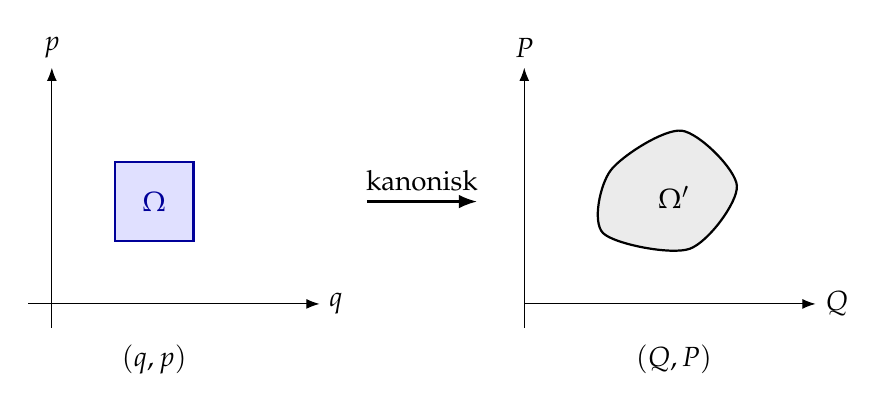
\begin{tikzpicture}[scale=1.0]
    \draw[-{Latex}] (-0.3,0) -- (3.4,0) node[right] {$q$};
    \draw[-{Latex}] (0,-0.3) -- (0,3.0) node[above] {$p$};
    \draw[thick,blue!60!black,fill=blue!12] (0.8,0.8) rectangle (1.8,1.8);
    \node[blue!60!black] at (1.3,1.3) {$\Omega$};
    \node at (1.3,-0.7) {$(q,p)$};

    \draw[-{Latex},thick] (4.0,1.3) -- (5.4,1.3) node[midway,above] {kanonisk};

    \draw[-{Latex}] (6.0,0) -- (9.7,0) node[right] {$Q$};
    \draw[-{Latex}] (6.0,-0.3) -- (6.0,3.0) node[above] {$P$};
    \draw[thick,black,fill=black!8] plot[smooth cycle] coordinates
      {(7.0,0.9) (8.1,0.7) (8.7,1.5) (8.0,2.2) (7.1,1.7)};
    \node at (7.9,1.35) {$\Omega'$};
    \node at (7.9,-0.7) {$(Q,P)$};
  \end{tikzpicture}
  \caption{En kanonisk transformation kan forvrænge et område $\Omega$ i
  faserummet ganske voldsomt i form — men arealet (i to dimensioner)
  hhv.\ volumenet (i $2n$ dimensioner) er altid bevaret, ligesom under
  den rene tidsudvikling i Liouvilles sætning
  (figur~\ref{fig:liouville}).}
  \label{fig:kanonisk-transf}
\end{figure}

\section{Opsummering}

\begin{itemize}
  \item En kanonisk transformation $(q,p)\to(Q,P)$ er en transformation,
        der bevarer Hamiltons ligningers form, med en ny
        Hamilton-funktion $K$.
  \item Sådanne transformationer frembringes af genererende funktioner
        $F$, defineret via
        $\sum_ip_i\dot q_i-H=\sum_iP_i\dot Q_i-K+dF/dt$.
  \item For $F_1(q,Q,t)$: $p_i=\partial F_1/\partial q_i$,
        $P_i=-\partial F_1/\partial Q_i$, $K=H+\partial F_1/\partial t$.
  \item For $F_2(q,P,t)=F_1+\sum_iQ_iP_i$: $p_i=\partial F_2/\partial q_i$,
        $Q_i=\partial F_2/\partial P_i$, $K=H+\partial F_2/\partial t$
        — den type, vi primært bruger fremover.
  \item En infinitesimal kanonisk transformation genereret af $G$
        giver $\delta f=\varepsilon\{f,G\}$; specielt genererer $H$
        selv (med $\varepsilon=dt$) den faktiske tidsudvikling.
  \item Kanoniske transformationer bevarer alle Poisson-parenteser —
        Poisson-strukturen er en invariant egenskab af faserummet, ikke
        af et bestemt koordinatvalg.
\end{itemize}

\begin{opgave}
Vis, at variation af $S=\int(\sum_ip_i\dot q_i-H)\,dt$ med hensyn til
uafhængige, arbitrære $\delta q_i(t)$ og $\delta p_i(t)$ (begge nul
ved endepunkterne $t_1,t_2$ for $\delta q_i$; ingen randbetingelse er
nødvendig for $\delta p_i$, da der ikke integreres partielt i $p_i$)
giver netop Hamiltons ligninger \eqref{eq:hamiltons-ligninger} som
Euler-Lagrange-ligninger.
\end{opgave}

\begin{opgave}
Udfør mellemregningen, der fører fra $F_1$-relationerne
\eqref{eq:F1-relationer} til $F_2$-relationerne
\eqref{eq:F2-relationer}, ved at differentiere
$F_2=F_1+\sum_iQ_iP_i$ totalt og sammenligne med
\eqref{eq:genererende-betingelse} skrevet om for $F_2$.
\end{opgave}

\begin{opgave}
Bekræft for eksemplet $Q_i=p_i$, $P_i=-q_i$, at de fundamentale
Poisson-parenteser \eqref{eq:kanonisk-poisson-betingelse} er opfyldt
(udregnet med hensyn til de gamle variable $(q,p)$), og vis, at
transformationen \emph{uden} minustegnet (dvs.\ $Q_i=p_i,P_i=q_i$)
ville bryde $\{Q_i,P_i\}=\delta_{ij}$.
\end{opgave}

\begin{opgave}
Lad $G=H$ selv være generator af en infinitesimal transformation med
$\varepsilon=dt$, og brug \eqref{eq:infinitesimal-generator} med
$f=q_i$ og $f=p_i$ til at genfinde Hamiltons ligninger. Diskuter,
hvorfor dette bekræfter påstanden i bemærkningen om, at ``tidsudvikling
er en kanonisk transformation genereret af $H$''.
\end{opgave}


% --- Del II: Hamilton-Jacobi-teori ---
\part{Hamilton-Jacobi-teori}
% kap06.tex — Hamilton-Jacobi-teori
% Hamilton-Jacobi-kompendiet

\chapter{Hamilton-Jacobi-teori}
\label{kap:hj}

Dette kapitel er kompendiets omdrejningspunkt. Alt det foregående —
Lagrange- og Hamilton-formalismen, Poisson-parenteser, kanoniske
transformationer — har været forberedelse til netop dette skridt:
at finde den kanoniske transformation, der gør dynamikken så simpel,
som den overhovedet kan blive.

\section{Strategien: transformer bevægelsen væk}

I bemærkningen sidst i afsnit~\ref{sec:hamiltons-princip}-diskussionen
i kapitel~\ref{kap:kanoniske-transf} så vi, at tidsudviklingen selv kan
opfattes som en kanonisk transformation, genereret af $H$. Dette
antyder en dristig idé: hvad hvis vi søger en kanonisk transformation
$(q,p)\to(Q,P)$, hvor den \emph{nye} Hamilton-funktion $K$ er identisk
nul?

Hvis $K\equiv 0$, siger Hamiltons ligninger i de nye variable
\eqref{eq:hamilton-nye-var} simpelthen
\begin{equation}
  \dot Q_i = \pdv{K}{P_i} = 0, \qquad \dot P_i = -\pdv{K}{Q_i} = 0.
\end{equation}
Både $Q_i$ og $P_i$ er altså \emph{konstante} — vi skriver
$Q_i=\beta_i$, $P_i=\alpha_i$, hvor $\alpha_i,\beta_i$ er $2n$
konstanter, bestemt af begyndelsesbetingelserne. Al den dynamiske
information om systemet er dermed flyttet over i selve
transformationen: at finde bevægelsen $q_i(t)$ er reduceret til at
finde \emph{transformationen} — dvs.\ den genererende funktion — der
opnår $K\equiv 0$. Dette er den \emph{eneste} idé i Hamilton-Jacobi-
teorien; resten af kapitlet handler om at gøre den eksplicit.

\section{Udledning af Hamilton-Jacobi-ligningen}

Vi søger transformationen via en genererende funktion af type $F_2$
(afsnit~\ref{kap:kanoniske-transf}'s notation), som vi her — af
historiske og notationsmæssige grunde — kalder $S(q,t)$ i stedet for
$F_2(q,P,t)$, og hvor vi lader $S$ afhænge af $n$ konstanter
$\alpha_1,\dots,\alpha_n$, som spiller rollen af de nye impulser $P_i$:
\begin{equation}
  S = S(q_1,\dots,q_n,\alpha_1,\dots,\alpha_n,t).
\end{equation}
Ifølge de $F_2$-relationer, vi udledte i \eqref{eq:F2-relationer}
(med $P_i\to\alpha_i$), er
\begin{equation}
  p_i = \pdv{S}{q_i}, \qquad Q_i = \pdv{S}{\alpha_i}, \qquad K = H + \pdv{S}{t}.
  \label{eq:S-relationer}
\end{equation}
Betingelsen $K\equiv 0$ giver derfor, ved indsættelse af den første
relation i $H$:
\begin{equation}
  \boxed{H\left(q_1,\dots,q_n,\pdv{S}{q_1},\dots,\pdv{S}{q_n},t\right) + \pdv{S}{t} = 0.}
  \label{eq:hj-ligning}
\end{equation}
Dette er \emph{Hamilton-Jacobi-ligningen}\index{Hamilton-Jacobi-ligningen}. Det er en enkelt
\emph{partiel} differentialligning, første ordens i tid og i hver
$q_i$, for den ukendte funktion $S(q,t)$ — i modsætning til Hamiltons
$2n$ almindelige, om end koblede, differentialligninger for
$(q_i(t),p_i(t))$. Funktionen $S$ kaldes \emph{Hamiltons\index{Hamiltons principfunktion}
principfunktion}.

\begin{bemaerkning}
Det virker måske som en dårlig handel at bytte $2n$ almindelige
differentialligninger ud med \'en partiel differentialligning — en
PDE er typisk sværere at løse end et system af ODE'er. Værdien af
Hamilton-Jacobi-ligningen ligger ikke i, at den generelt er lettere at
løse, men i, at den for en stor og vigtig klasse af systemer
(\emph{separable} systemer, se afsnit~\ref{sec:separation}) reducerer
til simple, en-variabel integraler — og i, at den giver et begrebsapparat
(virkningen $S$ som funktion af tilstand og tid), der overlever direkte
ind i kvantemekanikken, som vi antyder i afsnit~\ref{sec:hj-og-kvante}.
\end{bemaerkning}

\subsection{$S$ er virkningen}

Vi bekræfter, at $S$ virkelig er den samme størrelse, vi kaldte
virkningen i \eqref{eq:virkning}. Langs en faktisk løsning, hvor
$p_i=\partial S/\partial q_i$ (fra \eqref{eq:S-relationer}):
\begin{equation}
  \dv{S}{t} = \sum_i\pdv{S}{q_i}\dot q_i + \pdv{S}{t}
  = \sum_i p_i\dot q_i + \pdv{S}{t}
  = \sum_i p_i\dot q_i - H = L,
\end{equation}
hvor vi i næstsidste skridt brugte Hamilton-Jacobi-ligningen
\eqref{eq:hj-ligning} til at sætte $\partial S/\partial t=-H$, og i
sidste skridt brugte definitionen af $L$ fra Legendre-transformationen
\eqref{eq:def-H}. Vi finder altså $dS/dt = L$, hvilket ved integration
giver
\begin{equation}
  S = \int L\,dt + \text{konstant},
\end{equation}
netop virkningen \eqref{eq:virkning}, evalueret langs den faktiske
bane, som funktion af dens sluttidspunkt og -position. Dette er ikke
en tilfældig sammenfald af navne: Hamilton-Jacobi-ligningen er den
naturlige PDE-formulering af, at virkningen gør sig selv stationær.

\subsection{Den fulde (komplette) løsning og bevægelsen}

En løsning $S(q,\alpha,t)$ til \eqref{eq:hj-ligning}, som afhænger af
$n$ uafhængige konstanter $\alpha_1,\dots,\alpha_n$ på en sådan måde,
at Hesse-matricen $\partial^2S/\partial q_i\partial\alpha_j$ er
ikke-singulær, kaldes en \emph{komplet integral}\index{komplet integral} af
Hamilton-Jacobi-ligningen. (Bemærk: da kun \emph{afledte} af $S$
optræder i \eqref{eq:hj-ligning}, er $S$ i sig selv altid bestemt op
til en additiv konstant — denne tæller ikke som en af de $n$ ægte
$\alpha_i$'er.)

Givet en sådan komplet integral, giver den anden relation i
\eqref{eq:S-relationer} os direkte de $n$ resterende konstanter:
\begin{equation}
  \beta_i = \pdv{S}{\alpha_i}(q,\alpha,t).
  \label{eq:beta-relation}
\end{equation}
Dette er $n$ ligninger, der (i princippet) kan løses for
$q_1,\dots,q_n$ som funktion af $t$ og de $2n$ konstanter
$(\alpha,\beta)$ — og \emph{det} er selve løsningen til bevægelsen! Vi
opsummerer proceduren:

\begin{enumerate}
  \item Løs Hamilton-Jacobi-ligningen \eqref{eq:hj-ligning} for en
        komplet integral $S(q,\alpha,t)$.
  \item Beregn $\beta_i=\partial S/\partial\alpha_i$; sæt disse lig
        med konstanter, bestemt af begyndelsesbetingelserne.
  \item Løs de resulterende ligninger for $q_i(t)$.
  \item Find (om ønsket) $p_i(t)=\partial S/\partial q_i$, evalueret
        langs den fundne løsning.
\end{enumerate}

Denne procedure er hele Hamilton-Jacobi-metoden. Det eneste
resterende arbejde — som kan være betydeligt — er trin 1: at finde en
komplet integral. Vi vender os nu mod det vigtigste tilfælde, hvor
dette er muligt i praksis.

\section{Tidsuafhængigt $H$: separation i tiden}
\label{sec:separation}

Antag, at $H$ ikke afhænger eksplicit af $t$ (som i alle vores
eksempler hidtil). Vi ved fra kapitel~\ref{kap:hamilton}, at $H$ da er
en bevaret størrelse langs bevægelsen; kald denne bevarede værdi $E$
(typisk den mekaniske energi, jf.\ diskussionen efter
\eqref{eq:dHdt-generel}). Det er da naturligt at gætte på en løsning
af formen
\begin{equation}
  S(q,\alpha,t) = W(q,\alpha) - Et,
  \label{eq:S-separation-tid}
\end{equation}
hvor $E=E(\alpha)$ er en af konstanterne (eller en funktion af dem —
vi vælger simpelthen $\alpha_1\equiv E$). Indsat i
\eqref{eq:hj-ligning}, og da $\partial S/\partial q_i=\partial W/\partial q_i$
(det tidsafhængige led bidrager intet til de rumlige afledte):
\begin{equation}
  \boxed{H\left(q_1,\dots,q_n,\pdv{W}{q_1},\dots,\pdv{W}{q_n}\right) = E.}
  \label{eq:hj-tidsuafhaengig}
\end{equation}
Dette er den \emph{tidsuafhængige Hamilton-Jacobi-ligning}\index{Hamilton-Jacobi-ligningen!tidsuafhængig}, og $W$
kaldes \emph{Hamiltons karakteristiske funktion}\index{Hamiltons karakteristiske funktion}. Den er en PDE i de
rumlige variable alene — tiden er helt elimineret — hvilket typisk gør
den væsentligt lettere at løse end \eqref{eq:hj-ligning}.

\section{Eksempel: den harmoniske oscillator}

\begin{eksempel}
Vi løser den énddimensionale harmoniske oscillator
(jf.\ eksemplet i kapitel~\ref{kap:hamilton}) fuldstændigt via
Hamilton-Jacobi-metoden. Hamilton-funktionen er
\begin{equation}
  H = \frac{p^2}{2m} + \frac12 kx^2.
\end{equation}
Den tidsuafhængige Hamilton-Jacobi-ligning \eqref{eq:hj-tidsuafhaengig}
(med $p\to dW/dx$) bliver
\begin{equation}
  \frac{1}{2m}\left(\dv{W}{x}\right)^2 + \frac12 kx^2 = E
  \quad\Longrightarrow\quad
  \dv{W}{x} = \sqrt{2mE - mkx^2},
\end{equation}
hvor vi vælger den positive rod (svarende til bevægelse i positiv
$x$-retning; se bemærkningen nedenfor). Integration giver
\begin{equation}
  W(x,E) = \int\sqrt{2mE-mkx^2}\,dx,
\end{equation}
og dermed, ifølge \eqref{eq:S-separation-tid},
\begin{equation}
  S(x,E,t) = \int\sqrt{2mE-mkx^2}\,dx - Et.
\end{equation}
Vi finder $\beta$ ved \eqref{eq:beta-relation}, med $\alpha_1=E$:
\begin{equation}
  \beta = \pdv{S}{E} = \int\pdv{E}\sqrt{2mE-mkx^2}\,dx - t
        = \int\frac{m}{\sqrt{2mE-mkx^2}}\,dx - t.
\end{equation}
Skriv $a\equiv\sqrt{2E/k}$ (amplituden) og $\omega\equiv\sqrt{k/m}$
(vinkelfrekvensen, jf.\ kapitel~\ref{kap:hamilton}). Da
$2mE-mkx^2=mk(a^2-x^2)$, bliver integranden
\begin{equation}
  \frac{m}{\sqrt{mk(a^2-x^2)}} = \frac{1}{\omega}\cdot\frac{1}{\sqrt{a^2-x^2}},
\end{equation}
og standardintegralet $\int dx/\sqrt{a^2-x^2}=\arcsin(x/a)$ giver
\begin{equation}
  \beta = \frac{1}{\omega}\arcsin\left(\frac{x}{a}\right) - t.
\end{equation}
Løst for $x$:
\begin{equation}
  \boxed{x(t) = a\sin\bigl(\omega(t+\beta)\bigr),}
\end{equation}
den velkendte harmoniske bevægelse — udledt her fuldstændigt fra
Hamilton-Jacobi-ligningen, uden på noget tidspunkt at have opskrevet
eller løst Newtons eller Hamiltons differentialligninger direkte! Som
et sidste tjek: $p=\partial W/\partial x=\sqrt{2mE-mkx^2}=m a\omega\cos(\omega(t+\beta))$,
som netop stemmer med $p=m\dot x$ udregnet fra $x(t)$ ovenfor.

\begin{bemaerkning}
Fortegnsvalget for kvadratroden i $dW/dx$ svarer til, at $W$ (og dermed
$S$) kun er defineret entydigt inden for én ``gren'' af bevægelsen (fx
mens $x$ vokser). Ved vendepunkterne $x=\pm a$, hvor $p=0$, skal man i
princippet skifte til den anden gren. Dette tekniske punkt bliver
vigtigt, når vi i kapitel~\ref{kap:virkning-vinkel} indfører
virkningsvariable, som netop er konstrueret til at give en glat,
global beskrivelse hen over sådanne vendepunkter.
\end{bemaerkning}
\end{eksempel}

\section{Det geometriske billede: $S$ som en ``bølgefront''}

Der er en frugtbar geometrisk måde at tænke på Hamilton-Jacobi-
ligningen, som binder direkte tilbage til Fermats princip fra
kapitel~\ref{kap:newton-variation}. For fastholdt $t$ definerer
$S(q,t)=\text{konstant}$ en familie af ``overflader'' (kurver, for
$n=1$; hyperflader for større $n$) i konfigurationsrummet — analogt til
\emph{bølgefronter}\index{bølgefront} i optikken. Bevægelsens impuls $p_i=\partial S/\partial q_i$
er, geometrisk set, normalvektoren til disse overflader — ganske som
lysstråler i geometrisk optik altid står vinkelret på bølgefronterne.
Partiklens faktiske bane $q_i(t)$ krydser derfor altid
$S$-overfladerne vinkelret, og bevæger sig fra overflade til overflade,
efterhånden som $t$ (og dermed værdien af $S$ langs banen) vokser.

\begin{figure}[htbp]
  \centering
  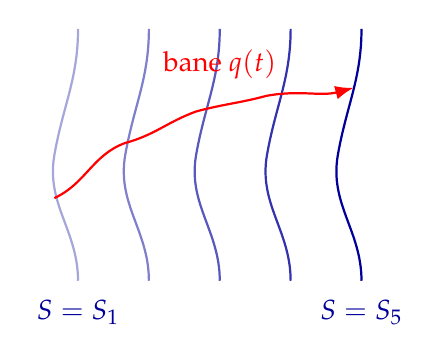
\begin{tikzpicture}[scale=1.0]
    % ``Bølgefronter'' = niveaukurver for S ved stigende tidspunkter
    \foreach \x/\op in {0.4/0.35,1.3/0.5,2.2/0.65,3.1/0.8,4.0/1.0} {
      \draw[thick,blue!60!black,opacity=\op]
        (\x,-1.6) to[out=90,in=-100] (\x-0.3,0) to[out=80,in=-90] (\x,1.6);
    }
    \node[blue!60!black] at (0.4,-2.0) {$S=S_1$};
    \node[blue!60!black] at (4.0,-2.0) {$S=S_5$};
    % Bane, der krydser bølgefronterne vinkelret
    \draw[-{Latex},thick,red] (0.1,-0.55) to[out=25,in=200] (1.0,0.15)
      to[out=15,in=200] (1.9,0.55) to[out=15,in=195] (2.8,0.75)
      to[out=10,in=195] (3.9,0.85);
    \node[red] at (2.2,1.15) {bane $q(t)$};
  \end{tikzpicture}
  \caption{Det geometriske billede af Hamilton-Jacobi-teorien: kurverne
  af konstant $S$ (blå, ``bølgefronter'', ved stigende værdier fra
  venstre mod højre) og partiklens faktiske bane (rød), som altid
  krydser dem vinkelret — impulsen $p=\partial S/\partial q$ er netop
  normalvektoren til fronterne. Sammenlign med bølgefronter og
  lysstråler i geometrisk optik, og med Fermats princip
  (kapitel~\ref{kap:newton-variation}).}
  \label{fig:hj-boelgefront}
\end{figure}

\section{Udblik: fra Hamilton-Jacobi til kvantemekanik}
\label{sec:hj-og-kvante}

Det geometriske billede i forrige afsnit er ikke kun en pædagogisk
analogi — det er historisk og begrebsmæssigt selve broen til
kvantemekanikken. I bølgeoptik er geometrisk optik (stråler vinkelret
på bølgefronter) en \emph{grænse}, gyldig når bølgelængden er meget
kort i forhold til systemets øvrige længdeskalaer; den fulde teori er
en bølgeligning for et felt, hvis faser netop svarer til $S$.

Schrödingers indsigt — som vi ikke udleder her, men blot antyder, og
som behandles fra den kvantemekaniske side i
[[kvantemekanik-kompendiet]] — var, at klassisk mekanik forholder sig
til en underliggende bølgeteori (kvantemekanikken) på præcis samme
måde, som geometrisk optik forholder sig til bølgeoptik. Skriver man
bølgefunktionen som $\psi=e^{iS/\hbar}$ og indsætter i Schrödinger-
ligningen, genfinder man i grænsen $\hbar\to0$ netop
Hamilton-Jacobi-ligningen \eqref{eq:hj-ligning} for $S$ — den klassiske
bevægelse er ``korthed-af-bølgelængde''-grænsen af kvantemekanikken, med
$S/\hbar$ som bølgens fase. Dette er den dybeste grund til, at
Hamilton-Jacobi-formalismen — i modsætning til Newtons eller endda
Hamiltons ligninger direkte — er den formulering af klassisk mekanik,
der mest gennemsigtigt viser, hvor kvantemekanikken ``kommer fra''.

\begin{bemaerkning}
Denne forbindelse — kaldet \emph{WKB-approksimationen}\index{WKB-approksimation} eller den
\emph{semiklassiske grænse}\index{semiklassisk grænse} — er et helt studieområde i sig selv, med
anvendelser fra tunnelering til Bohr-Sommerfeld-kvantisering.
Sidstnævnte er netop emnet for det næste kapitels afsluttende del
(kapitel~\ref{kap:adiabatisk}), hvor vi ser, hvordan virknings-
vinkel-variable (kapitel~\ref{kap:virkning-vinkel}) fører direkte til
den ældre kvanteteoris kvantiseringsbetingelser — det tankegods, der
var på plads, da kvantemekanikken blev født, og som er dette
kompendiums endestation.
\end{bemaerkning}

\section{Opsummering}

\begin{itemize}
  \item Strategien: find en kanonisk transformation til
        $K\equiv 0$, hvorved de nye variable $Q_i=\beta_i$,
        $P_i=\alpha_i$ bliver konstanter.
  \item Med genererende funktion $S(q,\alpha,t)$ af type $F_2$ giver
        $K=H+\partial S/\partial t=0$ Hamilton-Jacobi-ligningen
        $H(q,\partial S/\partial q,t)+\partial S/\partial t=0$.
  \item $S$ er (op til en konstant) selve virkningen: $dS/dt=L$.
  \item En komplet integral $S(q,\alpha,t)$ giver bevægelsen direkte
        via $\beta_i=\partial S/\partial\alpha_i$, løst for $q_i(t)$.
  \item Når $H$ er tidsuafhængig: $S=W(q,\alpha)-Et$, med $W$
        (Hamiltons karakteristiske funktion) løsning til den
        tidsuafhængige Hamilton-Jacobi-ligning
        $H(q,\partial W/\partial q)=E$.
  \item Geometrisk: $S=\text{konstant}$-flader er ``bølgefronter'', og
        banen krydser dem vinkelret med $p=\partial S/\partial q$ som
        normalvektor — analogt til geometrisk optik, og forløber for
        den semiklassiske grænse af kvantemekanikken ($\psi\sim e^{iS/\hbar}$).
\end{itemize}

\begin{opgave}
Løs den tidsuafhængige Hamilton-Jacobi-ligning for en fri partikel i
én dimension, $H=p^2/2m$, og vis, at proceduren giver den forventede
løsning $x(t)=x_0+\frac{p_0}{m}t$.
\end{opgave}

\begin{opgave}
Betragt en partikel, der falder frit i et konstant tyngdefelt,
$H=p^2/2m+mgx$ (med $x$ målt opad). Opstil og løs den tidsuafhængige
Hamilton-Jacobi-ligning, og genfind $x(t)=x_0+v_0t-\frac12gt^2$ ved
proceduren i afsnit~\ref{sec:separation}.
\end{opgave}

\begin{opgave}
Bekræft ved direkte differentiation, at $p=\partial W/\partial x=
\sqrt{2mE-mkx^2}$ og $x(t)=a\sin(\omega(t+\beta))$ (fra eksemplet med
den harmoniske oscillator) tilsammen opfylder $p=m\dot x$, og at
$H=p^2/(2m)+\frac12kx^2=E$ er opfyldt identisk for alle $t$.
\end{opgave}

% kap07.tex — Virknings-vinkel-variable
% Hamilton-Jacobi-kompendiet

\chapter{Virknings-vinkel-variable}
\label{kap:virkning-vinkel}

\section{Motivation: periodiske systemer uden fuld løsning}

I kapitel~\ref{kap:hj} løste vi den harmoniske oscillator ved at
integrere den tidsuafhængige Hamilton-Jacobi-ligning helt igennem for
at finde $W(x,E)$, og derefter differentiere med hensyn til $E$ for at
finde bevægelsen. Denne fulde løsning gav os $x(t)$ eksplicit — men den
kræver, at vi rent faktisk kan udføre integralet og derefter
\emph{invertere} resultatet for $x(t)$, hvad der langt fra altid er
muligt i lukket form.

For \emph{periodiske} systemer (og alle vores eksempler til videre er
periodiske eller kvasi-periodiske bevægelser i én frihedsgrad) findes
der en mellemvej, som giver os de fysisk vigtigste størrelser —
navnlig svingningsfrekvenserne — uden at kræve den fulde inversion.
Dette er \emph{virknings-vinkel-variablene}\index{virknings-vinkel-variable}. De er ikke kun et regne\-
teknisk trick: de er den formalisme, hvor den ældre kvanteteoris
kvantiseringsregler (kapitel~\ref{kap:adiabatisk}) tager deres mest
naturlige form.

\section{Klassifikation af periodisk bevægelse i én frihedsgrad}

Betragt et system med én frihedsgrad og tidsuafhængig $H(q,p)$. Banen i
faserummet $(q,p)$ — faseportrættet, jf.\ figur~\ref{fig:faseportraet}
— falder i to kvalitativt forskellige klasser:

\begin{itemize}
  \item \textbf{Libration}\index{libration}: banen er en lukket kurve i faserummet (som
        ellipserne for den harmoniske oscillator). Både $q$ og $p$ er
        periodiske funktioner af tiden med samme periode. Dette
        optræder typisk for bunden bevægelse i en potentialbrønd.
  \item \textbf{Rotation}\index{rotation (periodisk bevægelse)}: $p$ er en periodisk funktion af $q$, men
        $q$ selv vokser ubegrænset (som en vinkel, der løber
        rundt gentagne gange) — det klassiske eksempel er et
        pendul, der svinger hele vejen rundt i stedet for at
        oscillere, eller blot en fri partikel på en cirkel.
\end{itemize}

I begge tilfælde er $p(q)$ (banen i faserummet, ved fast $E$) en
\emph{periodisk} funktion af $q$, med en veldefineret periode i
$q$-retningen (for libration: hele svingningen; for rotation: én
omgang). Det er denne fælles egenskab, virknings-vinkel-formalismen
udnytter.

\section{Definition af virkningsvariablen}

For et system i én frihedsgrad definerer vi \emph{virkningsvariablen}\index{virkningsvariabel}
\begin{equation}
  \boxed{J \equiv \oint p\,dq,}
  \label{eq:def-J}
\end{equation}
hvor integralet tages over \'en fuld periode af bevægelsen: for
libration, hele vejen rundt om den lukkede faserumskurve; for
rotation, over ét fuldt gennemløb af $q$ (fx $0$ til $2\pi$ for en
vinkelvariabel). Da $p=\partial W/\partial q$ langs banen (fra
Hamilton-Jacobi-teorien i kapitel~\ref{kap:hj}), er $J$ funktionen af
energien $E$ alene:
\begin{equation}
  J(E) = \oint \pdv{W}{q}\,dq.
  \label{eq:J-fra-W}
\end{equation}
Geometrisk er $J/(2\pi)$ (eller, i visse konventioner, $J$ selv) netop
\emph{arealet}, som den lukkede faserumskurve indeslutter (for
librationstilfældet) — se figur~\ref{fig:virkningsareal}. Dette er en
direkte generalisering af det areal, vi allerede så for den harmoniske
oscillators ellipser i figur~\ref{fig:faseportraet}.

\begin{figure}[htbp]
  \centering
  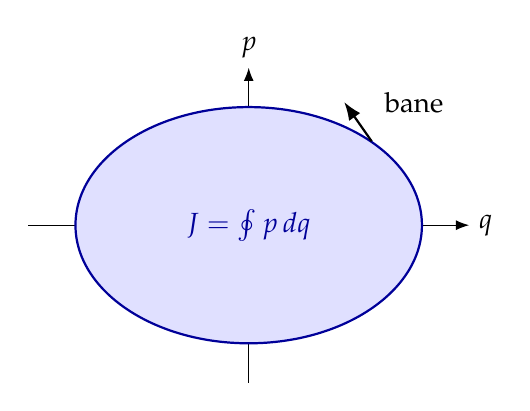
\begin{tikzpicture}[scale=1.0]
    \draw[-{Latex}] (-2.8,0) -- (2.8,0) node[right] {$q$};
    \draw[-{Latex}] (0,-2.0) -- (0,2.0) node[above] {$p$};
    \draw[thick,blue!60!black,fill=blue!12] (0,0) ellipse (2.2 and 1.5);
    \node[blue!60!black] at (0,0) {$J=\oint p\,dq$};
    \draw[-{Latex},thick] (2.2*0.71,1.5*0.71) -- (2.2*0.71-0.35,1.5*0.71+0.5);
    \node at (2.1,1.55) {bane};
  \end{tikzpicture}
  \caption{Virkningsvariablen $J=\oint p\,dq$ er (op til en faktor
  $2\pi$) arealet, som banen indeslutter i faserummet — her for
  libration (en lukket bane, som for den harmoniske oscillator).}
  \label{fig:virkningsareal}
\end{figure}

\section{Den konjugerede vinkelvariabel}

Da $J=J(E)$ (fra \eqref{eq:J-fra-W}) er en funktion af $E$ alene, kan
vi — i hvert fald i princippet — invertere den til $E=E(J)$, og
udtrykke Hamiltons karakteristiske funktion $W$ som funktion af $q$ og
$J$ i stedet for $q$ og $E$: $W=W(q,J)$. Vi udfører nu en kanonisk
transformation af type $F_2$ (kapitel~\ref{kap:kanoniske-transf}), med
$W(q,J)$ selv som genererende funktion, og med $J$ i rollen som den
nye impuls:
\begin{equation}
  p = \pdv{W}{q}, \qquad w \equiv \pdv{W}{J},
  \label{eq:def-w}
\end{equation}
hvor vi kalder den nye, konjugerede koordinat $w$ — \emph{vinkel\-
variablen}\index{vinkelvariabel}. Da $H=E=E(J)$ i disse variable ikke afhænger af $w$, giver
Hamiltons ligninger \eqref{eq:hamilton-nye-var} med $K=E(J)$:
\begin{equation}
  \dot J = -\pdv{E}{w} = 0, \qquad \dot w = \pdv{E}{J} \equiv \nu(J),
  \label{eq:hamilton-vinkel}
\end{equation}
hvor $\nu(J)\equiv dE/dJ$ er konstant i tiden (fordi $J$ selv er
konstant). Den anden ligning integreres trivielt:
\begin{equation}
  w(t) = \nu t + w_0.
  \label{eq:w-lineaer}
\end{equation}
Vinklen $w$ vokser altså \emph{lineært} med tiden — al den
tilsyneladende komplicerede periodiske bevægelse i $q$ er blevet
transformeret om til en variabel, der simpelthen løber rundt med
konstant hastighed $\nu$.

\subsection{$\nu$ er svingningsfrekvensen}

Vi viser nu, at $\nu$ netop er systemets \emph{svingningsfrekvens}\index{svingningsfrekvens} — hvilket
retfærdiggør navnet ``vinkelvariabel'' og gør hele konstruktionen
praktisk anvendelig. Betragt ændringen i $w$, når $q$ gennemløber netop
\'en fuld periode (defineret som i diskussionen omkring
\eqref{eq:def-J}):
\begin{equation}
  \Delta w \equiv \oint \pdv{w}{q}\,dq = \oint \pdv{}{q}\left(\pdv{W}{J}\right)dq
  = \dv{}{J}\oint \pdv{W}{q}\,dq = \dv{J}{J}\oint p\,dq\Big/ dJ,
\end{equation}
mere ligefremt: vi ombytter $\partial/\partial J$ og $\oint(\cdots)dq$
(tilladt, da integrationskonturen — én fuld periode i $q$ — ikke selv
afhænger af $J$), og bruger \eqref{eq:J-fra-W}:
\begin{equation}
  \Delta w = \dv{}{J}\oint\pdv{W}{q}\,dq = \dv{J}{J} = 1.
  \label{eq:delta-w-1}
\end{equation}
Vinkelvariablen $w$ vokser altså med præcis $1$ for hver fulde periode
af den oprindelige bevægelse i $q$. Sammenholdt med
\eqref{eq:w-lineaer}, hvor $w$ vokser lineært med hastighed $\nu$,
betyder dette, at perioden $\tau$ af den oprindelige bevægelse opfylder
$\nu\tau=1$, altså
\begin{equation}
  \boxed{\nu = \dv{E}{J} = \frac{1}{\tau}.}
  \label{eq:nu-er-frekvens}
\end{equation}
Dette er den centrale pointe i hele kapitlet: \emph{svingnings\-
frekvensen kan beregnes som $dE/dJ$, uden at vi nogensinde behøver
finde bevægelsen $q(t)$ eksplicit}. Vi skal blot kende $J$ som funktion
af $E$ — et almindeligt (ikke partielt) integral, jf.\
\eqref{eq:def-J} — og differentiere.

\section{Eksempel: den harmoniske oscillator, igen}

\begin{eksempel}
Vi genbesøger den harmoniske oscillator en tredje gang (jf.\
kapitel~\ref{kap:hamilton} og \ref{kap:hj}), nu via virknings-vinkel-
metoden. Faserumsbanen ved energi $E$ er ellipsen
$p^2/(2mE)+x^2/(2E/k)=1$ (fra kapitel~\ref{kap:hj}'s resultat
$x=a\sin(\omega(t+\beta))$, $p=ma\omega\cos(\omega(t+\beta))$, med
$a=\sqrt{2E/k}$). Virkningsvariablen \eqref{eq:def-J} er per
definition arealet af denne ellipse, ganget med $2\pi$ (se
figur~\ref{fig:virkningsareal}): en ellipse med halvakser
$a=\sqrt{2E/k}$ (i $x$-retningen) og $b=\sqrt{2mE}$ (i $p$-retningen)
har areal $\pi a b$, så
\begin{equation}
  J = \oint p\,dx = \pi ab = \pi\sqrt{\frac{2E}{k}}\sqrt{2mE} = 2\pi E\sqrt{\frac{m}{k}} = \frac{2\pi E}{\omega},
\end{equation}
hvor vi brugte $\omega=\sqrt{k/m}$. Løst for $E$:
\begin{equation}
  E(J) = \frac{\omega J}{2\pi} = \omega\left(\frac{J}{2\pi}\right).
\end{equation}
Frekvensen, ifølge \eqref{eq:nu-er-frekvens}, er
\begin{equation}
  \nu = \dv{E}{J} = \frac{\omega}{2\pi},
\end{equation}
netop svingningsfrekvensen $\nu=\omega/(2\pi)$ (i enheder af
svingninger pr.\ tidsenhed; $\omega$ selv er vinkelfrekvensen i
radianer pr.\ tidsenhed) — udledt uden på noget tidspunkt at have
integreret $dW/dx$ eksplicit, i modsætning til den fulde løsning i
kapitel~\ref{kap:hj}. Bemærk også formen $E=\nu J$ (med $\nu=\omega/2\pi$):
dette er den klassiske sammenhæng, der — som vi antyder i næste kapitel
— bliver til Plancks kvantiseringsbetingelse $E=nh\nu$, når $J$
begrænses til heltalsmultipla af Plancks konstant $h$.
\end{eksempel}

\section{Flere frihedsgrader: separable systemer}

Konstruktionen generaliseres til $n$ frihedsgrader, når
Hamilton-Jacobi-ligningen er \emph{fuldt separabel}: dvs.\ når man kan
finde en komplet integral af formen
\begin{equation}
  W(q_1,\dots,q_n,\alpha) = \sum_{i=1}^n W_i(q_i,\alpha),
\end{equation}
hvor hver $W_i$ kun afhænger af sin egen koordinat $q_i$ (og af de
$n$ konstanter $\alpha$ som parametre). Dette er tilfældet for alle
systemer, vi har mødt i kompendiet (fx central-kraft-problemet i
planpolar-koordinater, hvor $r$- og $\phi$-delen separerer, jf.\
opgaverne i kapitel~\ref{kap:lagrange} og \ref{kap:hamilton}).

For hvert sådant separabelt ``led'' defineres en egen virkningsvariabel
\begin{equation}
  J_i \equiv \oint p_i\,dq_i,
\end{equation}
hvor $p_i=\partial W_i/\partial q_i$, og integralet tages over den
periode, der er naturlig for netop koordinaten $q_i$ (som kan være
libration eller rotation, forskelligt for hver $i$). Hver $J_i$ har sin
egen konjugerede vinkelvariabel $w_i$, som vokser lineært med sin egen
frekvens $\nu_i=\partial E/\partial J_i$ — nu en \emph{partiel}
afledt, da $E=E(J_1,\dots,J_n)$ generelt afhænger af alle
virkningsvariablene. Systemets fulde bevægelse er dermed opløst i $n$
uafhængige, lineært voksende vinkler, hver med sin egen frekvens — en
\emph{multiperiodisk}\index{multiperiodisk bevægelse} bevægelse.

\begin{bemaerkning}
Dette er den klassiske forløber for begrebet ``normalmoder'' og for
kvantetalene $(n_1,\dots,n_n)$, der mærker de enkelte frihedsgrader i
et kvantiseret system (fx radial- og vinkelkvantetal for
hydrogenatomet). Vi forfølger denne parallel systematisk i næste
kapitel.
\end{bemaerkning}

\subsection{Det geometriske billede: bevægelsestorusen}

Det er værd at gøre sig det geometriske billede klart, fordi det er
selve grundstenen, som al senere teori om integrable og
ikke-integrable systemer bygger videre på. For \'en frihedsgrad
foregår bevægelsen på en lukket kurve i faserummet (figur~
\ref{fig:virkningsareal}) — topologisk en cirkel, parametriseret af
vinklen $w$. For $n$ frihedsgrader, med $n$ uafhængige
virkningsvariable $J_1,\dots,J_n$ alle konstante, foregår bevægelsen
tilsvarende på en $n$-dimensional \emph{torus}\index{bevægelsestorus} i faserummet: hver
vinkel $w_i\in[0,1)$ (eller $[0,2\pi)$, afhængig af konvention) er en
uafhængig cirkulær koordinat på torusen, og systemets tilstand
$(w_1,\dots,w_n)$ løber rundt på den med konstante hastigheder
$\nu_1,\dots,\nu_n$ — se figur~\ref{fig:torus} for $n=2$.

\begin{figure}[htbp]
  \centering
  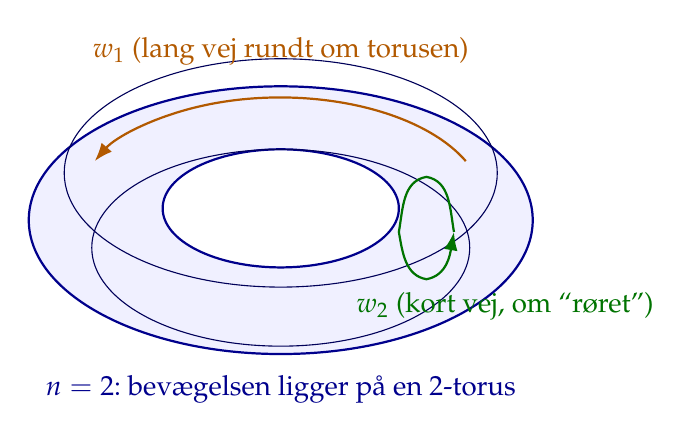
\begin{tikzpicture}[scale=1.0]
    % Torus (2D projektion): ydre og indre kontur
    \draw[thick,blue!55!black,fill=blue!6] (0,0) ellipse (3.2 and 1.7);
    \draw[thick,blue!55!black,fill=white] (0,0.15) ellipse (1.5 and 0.75);
    % Antydning af "rørets" runding med et par ekstra tynde ellipser
    \draw[blue!35!black,thin] (0,-0.35) ellipse (2.4 and 1.25);
    \draw[blue!35!black,thin] (0,0.6) ellipse (2.75 and 1.45);
    % w_1: "lang vej rundt" (den store cirkel)
    \draw[-{Latex},orange!70!black,thick] (2.35,0.75) arc[start angle=25,end angle=155,x radius=2.6,y radius=1.4];
    \node[orange!70!black] at (0,2.15) {$w_1$ (lang vej rundt om torusen)};
    % w_2: "kort vej rundt" (om røret) - antydet ved en lille lukket kurve
    \draw[-{Latex},green!45!black,thick] (2.2,-0.15) to[out=100,in=-10] (1.85,0.55) to[out=190,in=80] (1.5,-0.15) to[out=-80,in=170] (1.85,-0.75) to[out=10,in=-100] (2.2,-0.15);
    \node[green!45!black] at (2.85,-1.1) {$w_2$ (kort vej, om ``røret'')};
    \node[blue!55!black] at (0,-2.15) {$n=2$: bevægelsen ligger på en 2-torus};
  \end{tikzpicture}
  \caption{For $n$ separable frihedsgrader ligger bevægelsen på en
  $n$-dimensional torus i faserummet (her $n=2$), med hver
  vinkelvariabel $w_i$ som en uafhængig cirkulær koordinat. Er
  frekvenserne $\nu_1,\dots,\nu_n$ \emph{inkommensurable} (deres
  forhold er irrationale), fylder banen hele torusen tæt op
  (\emph{kvasiperiodisk} bevægelse); er de \emph{kommensurable}
  (rationalt forhold), lukker banen sig selv efter endeligt mange
  omløb (\emph{resonans}).}
  \label{fig:torus}
\end{figure}

Sondringen mellem \emph{kommensurable} og \emph{inkommensurable}
frekvenser, nævnt i figurteksten, er ikke en teknisk fodnote — det er
selve nålepunktet, hvor den pæne, fuldstændigt løselige verden, dette
kapitel beskriver, begynder at gå i stykker: perturberes et
integrabelt system svagt, er det netop de \emph{resonante} tori
(kommensurable frekvensforhold) der er skrøbelige og typisk opløses i
kaotisk bevægelse, mens de tilstrækkeligt \emph{ikke-resonante} tori
overlever (om end let deformerede) — indholdet af
Kolmogorov-Arnold-Moser-sætningen (KAM-sætningen). Dette er
selve udgangspunktet for et separat kompendium om kaos og
ikke-lineær dynamik.

\section{Eksempel: Kepler-problemet — flere frihedsgrader og degeneration}
\label{sec:kepler-action-angle}

\begin{eksempel}
Vi regner nu et fuldstændigt eksempel med $n=2$ frihedsgrader
igennem: en partikel med masse $m$, der bevæger sig i et
Kepler-/Coulomb-potentiale $V(r)=-k/r$ ($k>0$) i planpolar-koordinater
$(r,\phi)$. Hamilton-funktionen er
\begin{equation}
  H = \frac{p_r^2}{2m} + \frac{p_\phi^2}{2mr^2} - \frac{k}{r}.
\end{equation}
$\phi$ er cyklisk (jf.\ kapitel~\ref{kap:lagrange}), så $p_\phi=\ell$
(banemomentet) er en bevægelseskonstant, og
Hamilton-Jacobi-ligningen separerer fuldstændigt: $W=W_r(r)+\ell\phi$.
Vi har dermed to virkningsvariable, én for hver frihedsgrad.

\textbf{Den azimutale virkningsvariabel} er triviel, da $p_\phi=\ell$
er konstant, og $\phi$ er en \emph{rotationskoordinat} (den løber
rundt, $0$ til $2\pi$, for hvert omløb):
\begin{equation}
  J_\phi = \oint p_\phi\,d\phi = 2\pi\ell.
  \label{eq:kepler-Jphi}
\end{equation}

\textbf{Den radiale virkningsvariabel} kræver mere arbejde. For en
bunden bane ($E<0$) svinger $r$ periodisk (\emph{libration}) mellem et
minimum $r_{\min}$ og maksimum $r_{\max}$ (perihel og aphel), hvor
$p_r=\sqrt{2m\bigl(E+k/r\bigr)-\ell^2/r^2}=0$. Virkningsvariablen er
\begin{equation}
  J_r = \oint p_r\,dr = 2\int_{r_{\min}}^{r_{\max}}
    \sqrt{2mE + \frac{2mk}{r} - \frac{\ell^2}{r^2}}\;dr,
  \label{eq:kepler-Jr-integral}
\end{equation}
(faktor $2$, fordi $\oint$ dækker både ud- og indadgående bevægelse).
Dette er et standardintegral (løses fx ved konturintegration i det
komplekse $r$-plan, eller ved substitutionen $r=1/u$ efterfulgt af
kvadratkomplettering — se opgave nedenfor), med resultatet
\begin{equation}
  J_r = -2\pi\ell + 2\pi k\sqrt{\frac{m}{-2E}}.
  \label{eq:kepler-Jr}
\end{equation}
Læg mærke til, at $-2\pi\ell=-J_\phi$ indgår, jf.\
\eqref{eq:kepler-Jphi} — det er ingen tilfældighed: banemomentets
bidrag til den \emph{radiale} bevægelses ``omkreds'' i faserummet
skyldes centrifugalleddet $\ell^2/r^2$ i $p_r$, og forsvinder netop
med $J_\phi$'s eget bidrag, når vi lægger de to sammen.

\textbf{Degeneration: energien afhænger kun af summen $J_r+J_\phi$.}
Læg \eqref{eq:kepler-Jphi} og \eqref{eq:kepler-Jr} sammen:
\begin{equation}
  J \equiv J_r + J_\phi = 2\pi k\sqrt{\frac{m}{-2E}}.
\end{equation}
Løs for $E$:
\begin{equation}
  \boxed{E = -\frac{2\pi^2mk^2}{J^2} = -\frac{2\pi^2mk^2}{(J_r+J_\phi)^2}.}
  \label{eq:kepler-E-af-J}
\end{equation}
Dette er et bemærkelsesværdigt resultat: $E$ afhænger \emph{ikke} af
$J_r$ og $J_\phi$ hver for sig, kun af deres \emph{sum}. Systemet er
\emph{degenereret}\index{degeneration (virknings-vinkel-variable)}: de to frekvenser
\begin{equation}
  \nu_r = \pdv{E}{J_r} = \pdv{E}{J}, \qquad
  \nu_\phi = \pdv{E}{J_\phi} = \pdv{E}{J}
\end{equation}
er \emph{identiske}, $\nu_r=\nu_\phi$ — den radiale og den azimutale
bevægelse har nøjagtig samme periode, hvilket er præcis grunden til,
at Kepler-banen er en \emph{lukket} ellipse i stedet for en åben
rosette-bane (jf.\ Bertrands sætning, som siger, at kun
$V\propto1/r$ og $V\propto r^2$ giver lukkede baner for alle
energier). I torus-billedet fra figur~\ref{fig:torus} er
Kepler-banens torus derfor altid \emph{resonant} — den er et
grænsetilfælde af degeneration, ikke blot et specialtilfælde af et
kommensurabelt frekvensforhold.

\begin{bemaerkning}
Sæt Bohr-Sommerfeld-kvantiseringen $J_r=n_rh$, $J_\phi=n_\phi h$
($n_r=0,1,2,\dots$, $n_\phi=1,2,3,\dots$) ind i \eqref{eq:kepler-E-af-J}:
\begin{equation}
  E_n = -\frac{2\pi^2mk^2}{n^2h^2}, \qquad n\equiv n_r+n_\phi = 1,2,3,\dots
\end{equation}
Dette er, med $k=e^2/(4\pi\varepsilon_0)$, netop Bohrs formel for
hydrogenatomets energiniveauer (kompendiets ældre kvanteteori-kapitel,
kapitel~\ref{kap:adiabatisk}, viser metoden generelt; her ser vi dens
mest berømte anvendelse). At $E_n$ kun afhænger af \emph{summen}
$n=n_r+n_\phi$ — og altså er den samme for mange forskellige
kombinationer $(n_r,n_\phi)$ — er den klassiske forklaring på
hydrogenatomets berømte ``tilfældige'' (dynamiske) degeneration:
tilstande med samme $n$, men forskellig fordeling mellem radial og
azimutal bevægelse, har samme energi. Dette er intet mindre end
\emph{fordi} Kepler-banerne er lukkede, altså fordi torusen er
resonant for alle energier, ikke kun langs en isoleret
delmængde af dem. Den fulde kvantemekaniske forklaring på denne
degeneration (via en skjult $SO(4)$-symmetri for Coulomb-potentialet)
gives i [[kvantemekanik-kompendiet]].
\end{bemaerkning}

\begin{bemaerkning}
Dette eksempel illustrerer også, hvorfor degeneration er en
\emph{ikke-generisk} (skrøbelig) egenskab: den opstår her, fordi
$V\propto1/r$ er et af de meget få potentialer med ekstra, skjult
symmetri. Fjernes denne særlige struktur — fx ved at tilføje en lille
forstyrrelse til potentialet, $V(r)=-k/r+\varepsilon f(r)$ — ophæves
degenerationen typisk, $\nu_r\neq\nu_\phi$ for de fleste energier, og
banen bliver en åben rosette i stedet for en lukket ellipse. Hvad der
sker med de \emph{resonante} tori under en sådan forstyrrelse (som
her ligger tæt op ad hele torus-familien, ikke kun en tynd
delmængde) er netop det spørgsmål, KAM-sætningen og det planlagte
kaos-kompendium besvarer.
\end{bemaerkning}
\end{eksempel}

\section{Opsummering}

\begin{itemize}
  \item For periodiske systemer (libration eller rotation) i én
        frihedsgrad defineres virkningsvariablen $J=\oint p\,dq$
        — arealet (op til $2\pi$), som faserumsbanen indeslutter.
  \item $J=J(E)$; den konjugerede vinkelvariabel $w=\partial W/\partial J$
        vokser lineært med tiden, $w(t)=\nu t+w_0$, med
        $\nu=dE/dJ$.
  \item $\nu$ er præcis den fysiske svingningsfrekvens,
        $\nu=1/\tau$ — beregnet uden at skulle finde $q(t)$ eksplicit.
  \item For den harmoniske oscillator: $E(J)=\nu J$ med
        $\nu=\omega/(2\pi)$ — en form, der peger direkte mod Plancks
        kvantiseringsbetingelse.
  \item For separable systemer i flere frihedsgrader defineres en
        virkningsvariabel $J_i$ og frekvens $\nu_i=\partial E/\partial J_i$
        for hver koordinat, som løber uafhængigt og lineært; geometrisk
        ligger bevægelsen på en $n$-dimensional torus i faserummet.
  \item Er frekvenserne $\nu_i$ kommensurable, lukker banen sig selv
        (\emph{resonans}); er de inkommensurable, fylder den torusen
        tæt op (\emph{kvasiperiodisk}). Resonante tori er dem, der
        typisk opløses under en svag forstyrrelse — KAM-sætningens
        emne.
  \item Kepler-problemet ($V=-k/r$) er fuldt degenereret: $E$ afhænger
        kun af summen $J_r+J_\phi$, hvilket forklarer både banens
        lukkethed og hydrogenatomets ``tilfældige'' kvantedegeneration.
\end{itemize}

\begin{opgave}
En partikel med masse $m$ og energi $E$ bevæger sig frit (``rotation'')
på en cirkel med radius $R$ ($0\leq\phi<2\pi$, periodisk). Hamilton-
funktionen er $H=p_\phi^2/(2mR^2)$. Beregn $J=\oint p_\phi\,d\phi$
(integreret over $\phi\in[0,2\pi)$), find $E(J)$, og bekræft, at
$\nu=dE/dJ$ stemmer med den kendte omløbsfrekvens $v/(2\pi R)$, hvor
$v$ er partiklens (konstante) banehastighed.
\end{opgave}

\begin{opgave}
Vis, ved at differentiere \eqref{eq:def-w} med hensyn til tiden og
bruge kædereglen, at $\dot w = (\partial^2W/\partial q\partial J)\dot q$,
og brug dette sammen med \eqref{eq:hamilton-vinkel} til at genudlede
\eqref{eq:delta-w-1} på en alternativ måde: ved at integrere $\dot w$
over én fuld periode $\tau$ i $q$, og sammenholde med
$\Delta w = \nu\tau$.
\end{opgave}

\begin{opgave}
Udled \eqref{eq:kepler-Jr} fra integralet \eqref{eq:kepler-Jr-integral}.
Vink: substituér $u=1/r$ (så $dr=-du/u^2$), hvorved integranden
bliver kvadratroden af et andengradspolynomium i $u$; kvadratkomplettér
dette polynomium, brug standardresultatet
$\oint_{u_1}^{u_2}\sqrt{(u_2-u)(u-u_1)}\,du = \tfrac{\pi}{2}(u_2-u_1)$
(for \'et fuldt omløb, ud og tilbage), hvor $u_1,u_2$ er
polynomiets rødder — udtryk til sidst $u_1,u_2$ ved $m,E,\ell,k$
og reducér til \eqref{eq:kepler-Jr}. Alternativt: bekræft resultatet
numerisk for et selvvalgt talsæt $m,k,E,\ell$.
\end{opgave}


% --- Del III: Fra klassisk virkning til kvantefase ---
\part{Fra klassisk virkning til kvantefase}
% kap08.tex — Adiabatiske invarianter: broen til den ældre kvanteteori
% Hamilton-Jacobi-kompendiet

\chapter{Adiabatiske invarianter — broen til den ældre kvanteteori}
\label{kap:adiabatisk}

Dette kapitel er, sammen med kapitel~\ref{kap:felter-hamilton} (om
Hamiltonsk feltteori), et af de to kapitler, der udtrykkeligt peger
frem mod kompendiets endestation: det tankegods, der var på plads, da
kvantemekanikken blev født. Her når vi frem til selve
kvantiseringsbetingelsen fra ``den ældre kvanteteori'' (1900--1925) —
Bohr-Sommerfeld-kvantisering — som en næsten umiddelbar konsekvens af
virkningsvariablen $J$ fra kapitel~\ref{kap:virkning-vinkel}.

\section{Motivation: hvad sker der, når systemet ændres langsomt?}

Betragt et system, hvis Hamilton-funktion afhænger af en eller flere
ydre parametre — pendulets længde, kondensatorens pladeafstand,
beholderens rumfang — som ændres over tid, men \emph{langsomt} i
forhold til systemets egen svingningsperiode $\tau$. Vi skriver
Hamilton-funktionen som $H(q,p;\lambda(t))$, hvor $\lambda(t)$ er den
ydre parameter, og ``langsomt'' betyder præcist
\begin{equation}
  \left|\dv{\lambda}{t}\right|\cdot\tau \ll \lambda,
\end{equation}
altså at $\lambda$ ændrer sig kun ubetydeligt over en enkelt periode.
Et sådant system kaldes \emph{adiabatisk}\index{adiabatisk invarians} varierende — en betegnelse,
der (som i termodynamikken) betyder ``langsomt nok til, at systemet
ikke mærker forandringen fra et øjeblik til det næste'', ikke
nødvendigvis relateret til varmeisolation.

Spørgsmålet er: hvad sker der med virkningsvariablen $J$, når
$\lambda$ ændres på denne måde? Energien $E$ er bestemt \emph{ikke}
bevaret længere (systemet udveksler energi med det, der styrer
$\lambda$ — fx den hånd, der langsomt forkorter pendulets snor).
Svaret, vi udleder i næste afsnit, er overraskende robust: $J$ er
\emph{tilnærmelsesvis bevaret}, selv når $E$ ændrer sig betydeligt.

\section{Udledning af adiabatisk invarians}

Lad $J(E,\lambda)$ være virkningsvariablen \eqref{eq:def-J}, udregnet
ved en \emph{fastfrosset} værdi af $\lambda$ (dvs.\ langs den
faserumsbane, systemet ville følge, hvis $\lambda$ holdtes konstant på
sin nuværende værdi). Vi ønsker at vise, at den ægte tidsafledte af
$J$, \emph{gennemsnitliggjort over én svingningsperiode}, forsvinder
til første orden i $\dot\lambda$.

\subsection{Energiens ændring}

Langs den faktiske bevægelse er $H=H(q,p,\lambda(t))$, så den totale
tidsafledte af energien er (jf.\ \eqref{eq:dHdt-generel}, nu med
eksplicit tidsafhængighed via $\lambda(t)$ i stedet for direkte via
$t$):
\begin{equation}
  \dv{E}{t} = \pdv{H}{\lambda}\dot\lambda.
  \label{eq:dEdt-adiabatisk}
\end{equation}
Da $\lambda$ varierer langsomt, er $\dot\lambda$ tilnærmelsesvis
konstant over én periode $\tau$, og vi kan derfor gennemsnitliggøre
\eqref{eq:dEdt-adiabatisk} over en periode, med $\langle\cdot\rangle$
betegnende tidsgennemsnit:
\begin{equation}
  \left\langle\dv{E}{t}\right\rangle = \dot\lambda\left\langle\pdv{H}{\lambda}\right\rangle.
  \label{eq:dEdt-gennemsnit}
\end{equation}

\subsection{$J$'s afhængighed af $\lambda$ ved fast $E$}

Vi skal også kende, hvordan $J(E,\lambda)=\oint p\,dq$ ændrer sig, når
$\lambda$ ændres ved \emph{fast} $E$ (dvs.\ langs en anden frossen
bane, med samme energi men ny parameterværdi). Differentier
$H(q,p,\lambda)=E$ med hensyn til $\lambda$ ved fast $q$ og $E$:
\begin{equation}
  \pdv{H}{p}\pdv{p}{\lambda}\bigg|_{q,E} + \pdv{H}{\lambda}\bigg|_{q,p} = 0
  \quad\Longrightarrow\quad
  \pdv{p}{\lambda}\bigg|_{q,E} = -\dfrac{\partial H/\partial\lambda}{\partial H/\partial p} = -\dfrac{\partial H/\partial\lambda}{\dot q},
  \label{eq:dp-dlambda}
\end{equation}
hvor vi i sidste skridt brugte Hamiltons ligning $\dot q=\partial H/\partial p$.
Dermed:
\begin{equation}
  \pdv{J}{\lambda}\bigg|_E = \oint\pdv{p}{\lambda}\bigg|_{q,E}\,dq
  = -\oint\dfrac{\partial H/\partial\lambda}{\dot q}\,dq
  = -\oint\pdv{H}{\lambda}\,dt
  = -\tau\left\langle\pdv{H}{\lambda}\right\rangle,
  \label{eq:dJ-dlambda}
\end{equation}
hvor vi brugte $dq=\dot q\,dt$, og at integralet over én fuld periode
i $q$ svarer til integration over $t$ fra $0$ til $\tau$ — netop
$\tau$ gange tidsgennemsnittet.

\subsection{Sammenligning: $J$ er invariant}

$J(E,\lambda)$ er en funktion af to variable, så dens totale
tidsafledte er
\begin{equation}
  \dv{J}{t} = \pdv{J}{E}\dv{E}{t} + \pdv{J}{\lambda}\dot\lambda.
\end{equation}
Vi gennemsnitliggør over én periode, idet vi bruger, at $\partial J/\partial E$
og $\partial J/\partial\lambda$ selv varierer langsomt (de er
funktioner af de langsomt varierende $E$ og $\lambda$) og derfor kan
trækkes uden for gennemsnittet:
\begin{equation}
  \left\langle\dv{J}{t}\right\rangle
  = \pdv{J}{E}\left\langle\dv{E}{t}\right\rangle + \pdv{J}{\lambda}\dot\lambda.
\end{equation}
Vi indsætter nu \eqref{eq:dEdt-gennemsnit} og \eqref{eq:dJ-dlambda},
samt $\partial J/\partial E=1/\nu=\tau$ (fra
\eqref{eq:nu-er-frekvens}):
\begin{equation}
  \left\langle\dv{J}{t}\right\rangle
  = \tau\cdot\dot\lambda\left\langle\pdv{H}{\lambda}\right\rangle
    + \left(-\tau\left\langle\pdv{H}{\lambda}\right\rangle\right)\dot\lambda
  = 0.
  \label{eq:J-invariant-bevis}
\end{equation}
De to led ophæver hinanden \emph{identisk}. Dette er resultatet, vi
søgte:

\begin{center}
\emph{Virkningsvariablen $J$ er, gennemsnitligt over hver periode,
bevaret under langsomme (adiabatiske) ændringer af systemets
parametre — selvom energien $E$ generelt ændrer sig betydeligt.}
\end{center}

\begin{bemaerkning}
Beviset ovenfor er en plausibilitetsargumentation på det niveau, der
er sædvanligt i indførende fremstillinger (jf.\ Landaus \emph{Mechanics}),
og er ikke en fuldt rigorøs matematisk sætning: en fuldstændig
behandling skal vise, at afvigelserne fra invarians er af højere orden
i $\dot\lambda/\omega$ og ikke akkumulerer systematisk over mange
perioder. Vi nøjes her med resultatet i den form, der er nødvendig for
at forstå dets historiske og begrebsmæssige rolle.
\end{bemaerkning}

\section{Eksempel: oscillator med langsomt varierende frekvens}

\begin{eksempel}
For den harmoniske oscillator fandt vi i
kapitel~\ref{kap:virkning-vinkel}, at $J=2\pi E/\omega$. Er $\omega$
(fx fordi fjederkonstanten $k$ eller massen $m$ ændres langsomt) en
langsomt varierende parameter, siger adiabatisk invarians af $J$, at
\begin{equation}
  \frac{E}{\omega} = \text{konstant} \qquad\text{(adiabatisk)}.
\end{equation}
Gøres $\omega$ større (fx en snor, der gøres kortere, eller en fjeder,
der strammes), vokser $E$ proportionalt — svingningens amplitude
\emph{aftager} (da $E=\frac12kA^2\propto\omega^2A^2$, og
$E\propto\omega$ giver $A^2\propto1/\omega$, altså $A\propto1/\sqrt\omega$),
men netop på den måde, at $J$, og dermed antallet af ``virkningskvanta''
i systemet (som vi præciserer i næste afsnit), forbliver uændret.
Dette er præcis den klassiske mekanisme, der ligger bag et velkendt
fænomen: et pendul, hvis snor langsomt forkortes (fx ved at trække
snoren op gennem et lille hul), får en voksende svingningsfrekvens og
en aftagende amplitude, på en måde, der er forudsigelig alene fra
$E/\omega=\text{konstant}$, uden at løse bevægelsesligningen i detalje.
\end{eksempel}

\begin{figure}[htbp]
  \centering
  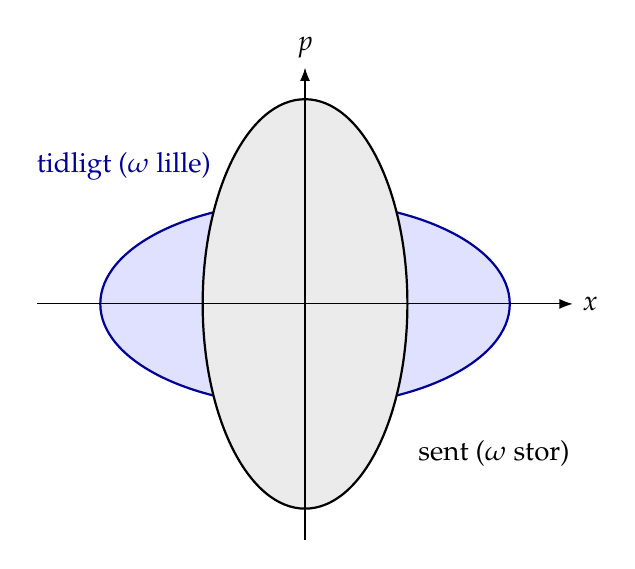
\begin{tikzpicture}[scale=1.0]
    % Oprindelig ellipse (lav omega, stor amplitude, moderat p)
    \draw[thick,blue!60!black,fill=blue!12] (0,0) ellipse (2.6 and 1.3);
    % Sen ellipse (høj omega, lille amplitude i x, stor i p) - samme areal
    \draw[thick,black,fill=black!8] (0,0) ellipse (1.3 and 2.6);
    % Akser og labels tegnes til sidst, så intet dækkes af ellipserne
    \draw[-{Latex}] (-3.4,0) -- (3.4,0) node[right] {$x$};
    \draw[-{Latex}] (0,-3.0) -- (0,3.0) node[above] {$p$};
    \node[blue!60!black] at (-2.3,1.75) {tidligt ($\omega$ lille)};
    \node at (2.4,-1.9) {sent ($\omega$ stor)};
  \end{tikzpicture}
  \caption{Adiabatisk invarians for oscillatoren: når $\omega$ langsomt
  vokser, ændrer faserumsellipsens form sig (amplituden i $x$
  aftager, i $p$ vokser) — men \emph{arealet}, altså $J$, forbliver
  uændret.}
  \label{fig:adiabatisk-ellipse}
\end{figure}

\section{Bohr-Sommerfeld-kvantiseringsbetingelsen}

Vi er nu ved kompendiets historiske og begrebsmæssige mål. I 1900
foreslog Planck, at strålingsenergien i en hulrumsresonator kun kunne
optræde i diskrete portioner $E=nh\nu$, hvor $\nu$ er frekvensen,
$h$ Plancks konstant, og $n$ et helt tal. Bohr udvidede i 1913 denne
idé til atomart bundne elektroner, og Sommerfeld (og uafhængigt
Wilson) generaliserede den i 1915--1916 til en systematisk regel for
\emph{alle} periodiske mekaniske systemer:

\begin{center}
\emph{Kun de baner, for hvilke virkningsvariablen opfylder}
\begin{equation}
  \boxed{J = \oint p\,dq = nh, \qquad n=0,1,2,\dots,}
  \label{eq:bohr-sommerfeld}
\end{equation}
\emph{er fysisk tilladte.}
\end{center}

Dette er \emph{Bohr-Sommerfeld-kvantiseringsbetingelsen}\index{Bohr-Sommerfeld-kvantisering}. Den centrale
pointe — og selve grunden til, at vi har brugt to fulde kapitler på at
udvikle virknings-vinkel-formalismen — er, at $J$ er netop den
størrelse, der (a) er en ren funktion af de klassiske
bevægelseskonstanter, og (b) er \emph{adiabatisk invariant}. Egenskab
(b) er afgørende: den betyder, at hvis et system langsomt forstyrres
(fx et atom, der langsomt bringes ind i et ydre felt), forbliver
kvantetallet $n$ det samme — kvantiseringen er robust over for
langsomme ydre ændringer, netop fordi den er formuleret via en
adiabatisk invariant og ikke via $E$ direkte.

\begin{bemaerkning}
Det er værd at være helt klar om, hvad denne ``ældre kvanteteori'' er,
og hvad den ikke er. Den er \emph{ikke} kvantemekanik i den moderne
betydning — der er ingen bølgefunktion, intet Hilbert-rum, ingen
operatorer. Den er en \emph{ad hoc}-regel, lagt oven på klassisk
mekanik, som (som vi ser i eksemplerne nedenfor) giver forbløffende
gode resultater for visse systemer, men fejler systematisk for andre
(den giver fx ingen korrekt beskrivelse af spektrallinjers intensitet,
og bryder sammen for mere komplicerede atomer end hydrogen). Dens
historiske betydning er, at den viste, at \emph{noget} i denne stil
måtte være rigtigt — og at dette ``noget'' senere blev identificeret som
den semiklassiske grænse af den fulde kvantemekanik (jf.\
afsnit~\ref{sec:hj-og-kvante} i kapitel~\ref{kap:hj}). Se
[[kvantemekanik-kompendiet]] for den fulde, korrekte teori.
\end{bemaerkning}

\section{Eksempel: kvantisering af den harmoniske oscillator}

\begin{eksempel}
For den harmoniske oscillator fandt vi $J=2\pi E/\omega$
(kapitel~\ref{kap:virkning-vinkel}). Bohr-Sommerfeld-betingelsen
\eqref{eq:bohr-sommerfeld} giver
\begin{equation}
  \frac{2\pi E_n}{\omega} = nh
  \quad\Longrightarrow\quad
  E_n = \frac{nh\omega}{2\pi} = nh\nu,
\end{equation}
hvor $\nu=\omega/(2\pi)$ er svingningsfrekvensen — netop Plancks
oprindelige kvantiseringsformel $E=nh\nu$! Dette er den historiske
kerne af hele udviklingen: Bohr-Sommerfeld-reglen \emph{reproducerer}
Plancks formel som et specialtilfælde, anvendt på den mekaniske
oscillator, i stedet for at postulere den for stråling alene.

Sammenlign nu med det korrekte kvantemekaniske resultat (udledt i
[[kvantemekanik-kompendiet]] ved at løse Schrödinger-ligningen for
oscillatoren):
\begin{equation}
  E_n^{\text{(korrekt)}} = \left(n+\frac12\right)h\nu, \qquad n=0,1,2,\dots
\end{equation}
De to resultater stemmer overens for \emph{energiforskellene} mellem
niveauer, $\Delta E=h\nu$, men Bohr-Sommerfeld-reglen mangler
nulpunktsenergien $\frac12h\nu$ — energien i grundtilstanden
($n=0$), som i den ældre teori forudsiges at være nul (ingen
bevægelse), men som i den korrekte kvantemekanik er strengt positiv
(en konsekvens af Heisenbergs usikkerhedsrelation: en partikel kan
ikke være fuldstændig i ro \emph{og} fuldstændig lokaliseret på
samme tid). Dette er et instruktivt eksempel på, hvor den ældre
kvanteteori går rigtigt (energikvantespring) og hvor den går forkert
(grundtilstandens energi) — begge dele klarlagt først med den fulde
kvantemekaniske behandling.
\end{eksempel}

\section{Eksempel: partikel i en kasse}

\begin{eksempel}
Betragt en partikel med masse $m$, der bevæger sig frit mellem to
uendeligt høje potentialvægge i $x=0$ og $x=L$ (en ``kasse'' eller
``boks''). Mellem væggene er $H=p^2/(2m)$, så ved energi $E$ er
$p=\pm\sqrt{2mE}$ — konstant numerisk værdi, med fortegnsskift ved hver
reflektion. Bevægelsen er libration: partiklen løber fra $0$ til $L$
og tilbage igen, hvilket giver virkningsvariablen som \emph{hele}
omløbet:
\begin{equation}
  J = \oint p\,dx = \int_0^L\sqrt{2mE}\,dx + \int_L^0\left(-\sqrt{2mE}\right)dx
    = 2L\sqrt{2mE}.
\end{equation}
Bohr-Sommerfeld-betingelsen $J=nh$ giver
\begin{equation}
  2L\sqrt{2mE_n} = nh
  \quad\Longrightarrow\quad
  \boxed{E_n = \frac{n^2h^2}{8mL^2}, \qquad n=1,2,3,\dots}
\end{equation}
(vi udelukker $n=0$, som ville give $E=0$, dvs.\ ingen bevægelse
overhovedet — et fysisk meningsløst resultat, som den ældre teori ikke
selv kan udelukke, men som vi forkaster ud fra fysisk sund fornuft).
Dette resultat er, i modsætning til oscillator-eksemplet ovenfor,
\textbf{eksakt} — det stemmer fuldstændigt overens med den korrekte
kvantemekaniske løsning af den uendelige potentialbrønd (se
[[kvantemekanik-kompendiet]]). Dette er ingen tilfældighed: for netop
dette system er den ``gamle'' og den ``nye'' teori i eksakt overensstemmelse,
fordi potentialet er så simpelt (konstant inden i brønden), at der
ingen krumning er i $p(x)$, som WKB-korrektionerne (jf.\
afsnit~\ref{sec:hj-og-kvante}) ellers ville skulle rette for.
\end{eksempel}

\section{Korrespondensprincippet}

De to eksempler ovenfor illustrerer et generelt mønster, formuleret af
Bohr som \emph{korrespondensprincippet}\index{korrespondensprincippet}: for store kvantetal $n$
nærmer de kvantemekaniske forudsigelser sig de klassiske. For
oscillatoren er den relative afvigelse mellem $E_n=nh\nu$ og
$E_n^{\text{korrekt}}=(n+\frac12)h\nu$ af størrelsesordnen $1/(2n)\to0$,
når $n\to\infty$. Mere generelt gælder, at forskellen mellem
successive kvantiserede energiniveauer, $\Delta E=E_{n+1}-E_n$, går mod
den klassiske svingningskvant $h\nu(E)$ — sammenlign med
\eqref{eq:nu-er-frekvens}, $\nu=dE/dJ$, som i kvantesproget netop
bliver $\Delta E/\Delta J$ med $\Delta J=h$.

\begin{bemaerkning}
Korrespondensprincippet er den sidste brik i broen fra klassisk
mekanik til kvantemekanik, som dette kompendium bygger. Vi har nu set
den i tre uafhængige, men sammenhængende former: (i) det geometriske
bølgefront-billede og $\psi\sim e^{iS/\hbar}$ fra
kapitel~\ref{kap:hj}, (ii) virkningsvariablens rolle som ``antal
kvanta gange $h$'' i dette kapitel, og (iii) korrespondensprincippets
udsagn, at kvantiseringens ``gitterafstand'' $\Delta E=h\nu$ bliver
relativt ubetydelig for store $n$, netop hvor klassisk mekanik er en
god beskrivelse. Den systematiske, korrekte udførelse af denne
overgang — med bølgefunktioner, operatorer og Hilbert-rum — er
[[kvantemekanik-kompendiet]]s emne. Dette kompendiums resterende
kapitler (9--10) fuldender i stedet den klassiske side af historien
ved at udvide formalismen til felter, som forberedelse til det senere
kvantefeltteori-kompendium.
\end{bemaerkning}

\section{Opsummering}

\begin{itemize}
  \item Et system, hvis parametre $\lambda(t)$ ændres langsomt
        ($\dot\lambda\tau\ll\lambda$) kaldes adiabatisk. Energien
        $E$ ændrer sig generelt, men virkningsvariablen $J$ er
        \emph{adiabatisk invariant}: $\langle dJ/dt\rangle=0$ til
        første orden i $\dot\lambda$.
  \item Beviset bruger $\partial J/\partial E=\tau$ og
        $\partial J/\partial\lambda|_E=-\tau\langle\partial H/\partial\lambda\rangle$,
        som tilsammen ophæver hinanden.
  \item For oscillatoren: $E/\omega$ er adiabatisk invariant.
  \item Bohr-Sommerfeld-kvantisering: $J=nh$ er den ældre kvanteteoris
        regel for, hvilke klassiske baner der er fysisk realiserede.
        Robustheden af $n$ under langsomme forstyrrelser er netop en
        konsekvens af $J$'s adiabatiske invarians.
  \item For oscillatoren giver reglen $E_n=nh\nu$ (Plancks formel),
        men mangler den korrekte kvantemekaniske nulpunktsenergi
        $\frac12h\nu$.
  \item For partiklen i kassen giver reglen det \emph{eksakte}
        kvantemekaniske resultat $E_n=n^2h^2/(8mL^2)$.
  \item Korrespondensprincippet: klassisk og kvantemekanisk beskrivelse
        falder sammen for store kvantetal $n$.
\end{itemize}

\begin{opgave}
Et pendul med masse $m$ svinger med lille udslag og længde $\ell(t)$,
der langsomt aftager med tiden (svingningsfrekvensen er
$\omega=\sqrt{g/\ell}$). Brug den adiabatiske invarians $E/\omega=\text{konstant}$
til at finde, hvordan svingningens amplitude $\theta_0$ afhænger af
$\ell$ (brug $E\approx\frac12m\ell^2\omega^2\theta_0^2$ for et
pendul med lille udslag).
\end{opgave}

\begin{opgave}
Genudled resultatet $E_n=n^2h^2/(8mL^2)$ for partiklen i kassen ved i
stedet at bruge det korrekte kvantemekaniske udtryk for de tilladte
bølgetal, $k_n=n\pi/L$ (stående bølger med noder ved $x=0,L$), og
$E_n=\hbar^2k_n^2/(2m)$, og bekræft, at de to fremgangsmåder giver
identisk resultat (brug $h=2\pi\hbar$).
\end{opgave}


% --- Del IV: Spredningsteori ---
% \part{Spredningsteori}

\backmatter
% \appendix

\end{document}
